%%%%%%%%%%%%%%%%%%%%%%%%%%%%%%%%%%%%%%%%%%%%%%%%%%%%%%%%%%%%%%%%%%%%%%%%%%%%%%
% CHAPTER 5
% SOFTWARE TESTING
%%%%%%%%%%%%%%%%%%%%%%%%%%%%%%%%%%%%%%%%%%%%%%%%%%%%%%%%%%%%%%%%%%%%%%%%%%%%%%

\chapter{SOFTWARE TESTING}

\section{Giới thiệu chương}

Kiểm thử phần mềm (Software Testing) là một trong những giai đoạn quan trọng trong vòng đời phát triển phần mềm, có vai trò đánh giá chất lượng của hệ thống trước khi đưa vào sử dụng. Mục đích của quá trình kiểm thử là xác minh rằng hệ thống đáp ứng đầy đủ các yêu cầu chức năng và phi chức năng đã được đặc tả, đồng thời phát hiện các lỗi còn tồn tại để kịp thời sửa chữa, nâng cao tính ổn định và độ tin cậy của sản phẩm.

Đối với dự án \textbf{SEAL Hackathon Management System}, quá trình kiểm thử được tiến hành sau khi hoàn thành các giai đoạn phân tích yêu cầu, thiết kế hệ thống và hiện thực các chức năng chính. Hệ thống được xây dựng nhằm hỗ trợ công tác quản lý cuộc thi Hackathon, bao gồm quản lý tài khoản, quản lý đội thi, quản lý thành viên và quản lý bài nộp dự án. Vì vậy, việc kiểm thử đóng vai trò quan trọng trong việc bảo đảm hệ thống hoạt động đúng với quy trình nghiệp vụ, đáp ứng yêu cầu sử dụng và hạn chế tối đa các lỗi có thể xảy ra trong quá trình vận hành.

Trong chương này, nhóm tiến hành kiểm thử trên toàn bộ các chức năng đã được triển khai trong hệ thống. Các trường hợp kiểm thử được xây dựng dựa trên tài liệu đặc tả yêu cầu phần mềm (Software Requirements Specification – SRS) và tài liệu thiết kế hệ thống (Software Design Description – SDD). Mỗi trường hợp kiểm thử đều xác định rõ dữ liệu đầu vào, các bước thực hiện, kết quả mong đợi và kết quả thực tế nhằm đánh giá mức độ đáp ứng của hệ thống.

Ngoài việc kiểm tra các chức năng hoạt động đúng theo yêu cầu, nhóm còn thực hiện kiểm thử đối với các trường hợp ngoại lệ như dữ liệu đầu vào không hợp lệ, truy cập trái phép, thao tác không đúng quyền hoặc các tình huống có thể ảnh hưởng đến tính toàn vẹn của dữ liệu. Điều này giúp hệ thống trở nên ổn định hơn và nâng cao trải nghiệm của người sử dụng.

Các nội dung chính được trình bày trong chương bao gồm mục tiêu kiểm thử, phạm vi kiểm thử, môi trường kiểm thử, phương pháp kiểm thử, thiết kế các trường hợp kiểm thử, kết quả kiểm thử thực tế cũng như những lỗi được phát hiện và biện pháp khắc phục trong quá trình phát triển hệ thống.

%%%%%%%%%%%%%%%%%%%%%%%%%%%%%%%%%%%%%%%%%%%%%%%%%%%%%%%%%%%%%%%%%%%%%%%%%%%%%%

\section{Mục tiêu kiểm thử}

\subsection{Mục tiêu tổng quát}

Mục tiêu tổng quát của quá trình kiểm thử là đánh giá mức độ đáp ứng của hệ thống \textbf{SEAL Hackathon Management System} đối với các yêu cầu đã được xác định trong quá trình phân tích và thiết kế. Thông qua hoạt động kiểm thử, nhóm mong muốn bảo đảm rằng tất cả các chức năng của hệ thống hoạt động đúng theo nghiệp vụ, dữ liệu được xử lý chính xác và hệ thống có thể vận hành ổn định trong môi trường thực tế.

Bên cạnh đó, kiểm thử còn giúp đánh giá khả năng phối hợp giữa các thành phần của hệ thống như giao diện người dùng (Frontend), dịch vụ xử lý nghiệp vụ (Backend) và cơ sở dữ liệu (Database), từ đó bảo đảm toàn bộ hệ thống hoạt động thống nhất và đồng bộ.

\subsection{Mục tiêu cụ thể}

Để đạt được mục tiêu tổng quát nêu trên, nhóm tiến hành kiểm thử nhằm thực hiện các mục tiêu cụ thể sau:

\begin{itemize}
	\item Kiểm tra tính chính xác của các chức năng đã được xây dựng theo yêu cầu của hệ thống.
	
	\item Kiểm tra quá trình xác thực người dùng thông qua cơ chế JWT Authentication.
	
	\item Đảm bảo dữ liệu người dùng được lưu trữ chính xác trong cơ sở dữ liệu SQLite.
	
	\item Kiểm tra tính hợp lệ của dữ liệu đầu vào tại cả phía giao diện và phía máy chủ.
	
	\item Đánh giá khả năng phân quyền giữa Trưởng đội và Thành viên trong quá trình sử dụng hệ thống.
	
	\item Kiểm tra việc thực thi các quy tắc nghiệp vụ như giới hạn số lượng thành viên, quyền tạo đội, quyền tham gia đội và quyền quản lý thành viên.
	
	\item Đảm bảo các RESTful API trả về đúng dữ liệu, đúng mã trạng thái HTTP và xử lý chính xác các trường hợp ngoại lệ.
	
	\item Kiểm tra khả năng đồng bộ dữ liệu giữa giao diện Dashboard và cơ sở dữ liệu sau mỗi thao tác của người dùng.
	
	\item Đánh giá khả năng hoạt động ổn định của hệ thống sau nhiều lần cập nhật dữ liệu liên tục.
	
	\item Phát hiện các lỗi còn tồn tại để tiến hành sửa chữa và hoàn thiện hệ thống trước khi triển khai.
\end{itemize}

Thông qua các mục tiêu trên, nhóm hướng đến việc xây dựng một hệ thống có tính ổn định cao, đáp ứng đúng yêu cầu nghiệp vụ của cuộc thi SEAL Hackathon và tạo nền tảng thuận lợi cho việc mở rộng trong các phiên bản tiếp theo.

%%%%%%%%%%%%%%%%%%%%%%%%%%%%%%%%%%%%%%%%%%%%%%%%%%%%%%%%%%%%%%%%%%%%%%%%%%%%%%

\section{Phạm vi kiểm thử}

\subsection{Phạm vi kiểm thử}

Hoạt động kiểm thử được thực hiện đối với toàn bộ các chức năng đã được triển khai trong phiên bản hiện tại của hệ thống. Các chức năng nằm trong phạm vi kiểm thử bao gồm:

\begin{itemize}
	\item Chức năng đăng ký tài khoản.
	
	\item Chức năng đăng nhập và đăng xuất hệ thống.
	
	\item Chức năng tạo đội thi Hackathon.
	
	\item Chức năng sinh mã mời của đội.
	
	\item Chức năng tham gia đội thông qua mã mời.
	
	\item Chức năng phê duyệt hoặc từ chối yêu cầu tham gia đội.
	
	\item Chức năng hiển thị danh sách thành viên của đội.
	
	\item Chức năng Kick thành viên khỏi đội.
	
	\item Chức năng thành viên rời khỏi đội.
	
	\item Chức năng giải tán đội.
	
	\item Chức năng nộp và cập nhật đường dẫn GitHub của dự án.
	
	\item Chức năng hiển thị Dashboard theo quyền của từng người dùng.
\end{itemize}

Ngoài các chức năng trên, nhóm cũng tiến hành kiểm thử quá trình trao đổi dữ liệu giữa Frontend và Backend nhằm bảo đảm các RESTful API hoạt động chính xác, dữ liệu được cập nhật đầy đủ và giao diện luôn phản ánh đúng trạng thái hiện tại của hệ thống.

\subsection{Phạm vi không kiểm thử}

Do giới hạn về thời gian và phạm vi của đồ án môn học, một số nội dung chưa được đưa vào kế hoạch kiểm thử của phiên bản hiện tại, bao gồm:

\begin{itemize}
	\item Kiểm thử hiệu năng với số lượng lớn người dùng truy cập đồng thời.
	
	\item Kiểm thử khả năng chịu tải của máy chủ trong môi trường triển khai thực tế.
	
	\item Kiểm thử bảo mật chuyên sâu bằng các công cụ phân tích lỗ hổng.
	
	\item Kiểm thử khả năng sao lưu và phục hồi dữ liệu khi xảy ra sự cố.
	
	\item Kiểm thử trên các nền tảng thiết bị di động chuyên dụng.
	
	\item Kiểm thử tích hợp với các hệ thống quản lý cuộc thi hoặc hệ thống chấm điểm tự động.
\end{itemize}

Những nội dung trên sẽ là cơ sở để nhóm tiếp tục nghiên cứu và phát triển trong các phiên bản mở rộng của hệ thống sau này.
%%%%%%%%%%%%%%%%%%%%%%%%%%%%%%%%%%%%%%%%%%%%%%%%%%%%%%%%%%%%%%%%%%%%%%%%%%%%%%
\section{Môi trường kiểm thử}
%%%%%%%%%%%%%%%%%%%%%%%%%%%%%%%%%%%%%%%%%%%%%%%%%%%%%%%%%%%%%%%%%%%%%%%%%%%%%%

\subsection{Môi trường phần cứng}

Quá trình kiểm thử được thực hiện trên máy tính cá nhân của nhóm phát triển. Cấu hình phần cứng đáp ứng yêu cầu triển khai hệ thống, đồng thời bảo đảm quá trình kiểm thử diễn ra ổn định. Thông tin về môi trường phần cứng được trình bày trong Bảng \ref{tab:hardware_environment}.

\begin{table}[H]
	\centering
	\caption{Môi trường phần cứng}
	\label{tab:hardware_environment}
	\renewcommand{\arraystretch}{1.3}
	\begin{tabular}{|p{5cm}|p{8cm}|}
		\hline
		\textbf{Thành phần} & \textbf{Thông số} \\
		\hline
		Hệ điều hành & Windows 11 64-bit \\
		\hline
		CPU & Intel Core i5 thế hệ 10 hoặc tương đương \\
		\hline
		RAM & 8 GB \\
		\hline
		Ổ cứng & SSD 512 GB \\
		\hline
		Kết nối mạng & Internet tốc độ cao \\
		\hline
	\end{tabular}
\end{table}

Việc kiểm thử được thực hiện trên cùng một môi trường phát triển với môi trường triển khai thử nghiệm nhằm giảm thiểu sự khác biệt trong quá trình đánh giá kết quả.

%%%%%%%%%%%%%%%%%%%%%%%%%%%%%%%%%%%%%%%%%%%%%%%%%%%%%%%%%%%%%%%%%%%%%%%%%%%%%%

\subsection{Môi trường phần mềm}

Trong quá trình phát triển và kiểm thử, nhóm sử dụng các công nghệ và thư viện hiện đại nhằm xây dựng một hệ thống có khả năng mở rộng, dễ bảo trì và đáp ứng tốt yêu cầu của cuộc thi Hackathon.

Bảng \ref{tab:software_environment} trình bày các thành phần phần mềm chính được sử dụng.

\begin{table}[H]
	\centering
	\caption{Môi trường phần mềm}
	\label{tab:software_environment}
	\renewcommand{\arraystretch}{1.3}
	\begin{tabular}{|p{5cm}|p{8cm}|}
		\hline
		\textbf{Thành phần} & \textbf{Phiên bản} \\
		\hline
		Python & 3.14 \\
		\hline
		FastAPI & 0.139.0 \\
		\hline
		Uvicorn & 0.51.0 \\
		\hline
		SQLAlchemy & 2.0.51 \\
		\hline
		SQLite & SQLite 3 \\
		\hline
		Passlib & 1.7.4 \\
		\hline
		BCrypt & 4.0.1 \\
		\hline
		python-jose & 3.3.0 \\
		\hline
		Pydantic & 2.13.4 \\
		\hline
		HTML5, CSS3, JavaScript & Frontend \\
		\hline
		Google Chrome & Trình duyệt kiểm thử \\
		\hline
		Visual Studio Code & IDE phát triển \\
		\hline
		GitHub & Quản lý mã nguồn \\
		\hline
		Ngrok & Triển khai thử nghiệm \\
		\hline
	\end{tabular}
\end{table}

Backend của hệ thống được triển khai bằng FastAPI kết hợp với Uvicorn. Frontend được xây dựng bằng HTML5, CSS3 và JavaScript thuần, giao tiếp với Backend thông qua các RESTful API.

%%%%%%%%%%%%%%%%%%%%%%%%%%%%%%%%%%%%%%%%%%%%%%%%%%%%%%%%%%%%%%%%%%%%%%%%%%%%%%

\subsection{Công cụ kiểm thử}

Để bảo đảm tính chính xác của kết quả kiểm thử, nhóm sử dụng nhiều công cụ hỗ trợ trong quá trình phát triển và đánh giá hệ thống.

\begin{table}[H]
	\centering
	\caption{Các công cụ hỗ trợ kiểm thử}
	\label{tab:test_tool}
	\renewcommand{\arraystretch}{1.3}
	\begin{tabular}{|p{4cm}|p{9cm}|}
		\hline
		\textbf{Công cụ} & \textbf{Mục đích sử dụng} \\
		\hline
		Swagger UI & Kiểm thử trực tiếp các RESTful API \\
		\hline
		Postman & Gửi Request và kiểm tra Response \\
		\hline
		Google Chrome DevTools & Kiểm tra Console, Network và Local Storage \\
		\hline
		SQLite Browser & Quan sát dữ liệu trong cơ sở dữ liệu \\
		\hline
		GitHub & Quản lý phiên bản mã nguồn \\
		\hline
		Ngrok & Kiểm thử truy cập từ Internet \\
		\hline
		Visual Studio Code & Chỉnh sửa và chạy chương trình \\
		\hline
	\end{tabular}
\end{table}

%%%%%%%%%%%%%%%%%%%%%%%%%%%%%%%%%%%%%%%%%%%%%%%%%%%%%%%%%%%%%%%%%%%%%%%%%%%%%%
\section{Phương pháp kiểm thử}
%%%%%%%%%%%%%%%%%%%%%%%%%%%%%%%%%%%%%%%%%%%%%%%%%%%%%%%%%%%%%%%%%%%%%%%%%%%%%%

Để đánh giá toàn diện chất lượng của hệ thống, nhóm áp dụng kết hợp nhiều phương pháp kiểm thử khác nhau. Mỗi phương pháp được sử dụng nhằm kiểm tra một khía cạnh cụ thể của phần mềm, từ chức năng nghiệp vụ cho đến giao diện người dùng và khả năng giao tiếp giữa các thành phần trong hệ thống.

%%%%%%%%%%%%%%%%%%%%%%%%%%%%%%%%%%%%%%%%%%%%%%%%%%%%%%%%%%%%%%%%%%%%%%%%%%%%%%

\subsection{Kiểm thử chức năng (Functional Testing)}

Kiểm thử chức năng được sử dụng để xác minh rằng tất cả các chức năng của hệ thống hoạt động đúng theo tài liệu đặc tả yêu cầu. Mỗi chức năng được xây dựng thành nhiều kịch bản kiểm thử với dữ liệu đầu vào khác nhau nhằm đánh giá khả năng xử lý của hệ thống.

Các chức năng chính được kiểm thử bao gồm:

\begin{itemize}
	\item Đăng ký tài khoản.
	\item Đăng nhập hệ thống.
	\item Tạo đội.
	\item Tham gia đội.
	\item Phê duyệt thành viên.
	\item Kick thành viên.
	\item Rời đội.
	\item Giải tán đội.
	\item Nộp bài dự thi.
	\item Đăng xuất hệ thống.
\end{itemize}

%%%%%%%%%%%%%%%%%%%%%%%%%%%%%%%%%%%%%%%%%%%%%%%%%%%%%%%%%%%%%%%%%%%%%%%%%%%%%%

\subsection{Kiểm thử hộp đen (Black-box Testing)}

Phương pháp Black-box Testing được áp dụng nhằm đánh giá hệ thống dựa trên dữ liệu đầu vào và kết quả đầu ra mà không quan tâm đến cấu trúc mã nguồn bên trong.

Người kiểm thử chỉ cần nhập dữ liệu, thực hiện các thao tác theo đúng quy trình sử dụng và so sánh kết quả thực tế với kết quả mong đợi. Đây là phương pháp phù hợp với các chức năng nghiệp vụ của hệ thống quản lý cuộc thi Hackathon.

%%%%%%%%%%%%%%%%%%%%%%%%%%%%%%%%%%%%%%%%%%%%%%%%%%%%%%%%%%%%%%%%%%%%%%%%%%%%%%

\subsection{Kiểm thử API}

Các RESTful API được kiểm thử thông qua Swagger UI và Postman.

Quá trình kiểm thử tập trung vào các nội dung sau:

\begin{itemize}
	\item Kiểm tra URL Endpoint.
	\item Kiểm tra phương thức HTTP.
	\item Kiểm tra Request Body.
	\item Kiểm tra Response JSON.
	\item Kiểm tra HTTP Status Code.
	\item Kiểm tra JWT Authentication.
	\item Kiểm tra phân quyền người dùng.
\end{itemize}

%%%%%%%%%%%%%%%%%%%%%%%%%%%%%%%%%%%%%%%%%%%%%%%%%%%%%%%%%%%%%%%%%%%%%%%%%%%%%%

\subsection{Kiểm thử giao diện người dùng}

Giao diện Dashboard được kiểm thử nhằm đánh giá khả năng hiển thị và phản hồi của hệ thống trên trình duyệt.

Các nội dung được kiểm tra bao gồm:

\begin{itemize}
	\item Hiển thị đúng thông tin tài khoản đăng nhập.
	\item Hiển thị đúng tên đội và mã mời.
	\item Ẩn hoặc hiện chức năng theo vai trò của người dùng.
	\item Cập nhật danh sách thành viên theo thời gian thực sau mỗi thao tác.
	\item Hiển thị thông báo lỗi và thông báo thành công chính xác.
	\item Điều hướng giữa các chức năng của Dashboard.
\end{itemize}

%%%%%%%%%%%%%%%%%%%%%%%%%%%%%%%%%%%%%%%%%%%%%%%%%%%%%%%%%%%%%%%%%%%%%%%%%%%%%%

\subsection{Kiểm thử tích hợp (Integration Testing)}

Sau khi các module được hoàn thành, nhóm tiến hành kiểm thử tích hợp nhằm đánh giá khả năng phối hợp giữa Frontend, Backend và cơ sở dữ liệu.

Các nội dung kiểm thử tích hợp bao gồm:

\begin{itemize}
	\item Frontend gửi Request đến Backend.
	\item Backend xử lý nghiệp vụ và truy cập cơ sở dữ liệu.
	\item SQLAlchemy thực hiện thao tác đọc và ghi dữ liệu.
	\item Backend trả về Response dưới dạng JSON.
	\item Frontend cập nhật giao diện theo dữ liệu nhận được.
\end{itemize}

Kết quả kiểm thử tích hợp cho thấy các thành phần của hệ thống phối hợp ổn định, dữ liệu được đồng bộ chính xác giữa giao diện người dùng và cơ sở dữ liệu, đáp ứng yêu cầu của hệ thống quản lý cuộc thi SEAL Hackathon.

%%%%%%%%%%%%%%%%%%%%%%%%%%%%%%%%%%%%%%%%%%%%%%%%%%%%%%%%%%%%%%%%%%%%%%%%%%%%%%
%%%%%%%%%%%%%%%%%%%%%%%%%%%%%%%%%%%%%%%%%%%%%%%%%%%%%%%%%%%%%%%%%%%%%%%%%%%%%%
\section{Thiết kế Test Case}
%%%%%%%%%%%%%%%%%%%%%%%%%%%%%%%%%%%%%%%%%%%%%%%%%%%%%%%%%%%%%%%%%%%%%%%%%%%%%%

Sau khi xác định được phạm vi và phương pháp kiểm thử, nhóm tiến hành xây dựng các trường hợp kiểm thử (Test Case) nhằm đánh giá toàn diện các chức năng của hệ thống. Mỗi Test Case được xây dựng dựa trên các yêu cầu chức năng đã được trình bày trong tài liệu SRS và phản ánh đúng quy trình nghiệp vụ của hệ thống quản lý cuộc thi SEAL Hackathon.

Các Test Case được thiết kế theo nguyên tắc mỗi trường hợp kiểm thử chỉ đánh giá một mục tiêu cụ thể. Điều này giúp việc xác định nguyên nhân khi xảy ra lỗi trở nên đơn giản hơn, đồng thời hỗ trợ quá trình bảo trì và mở rộng hệ thống trong tương lai.

Đối với mỗi chức năng, nhóm xây dựng đầy đủ điều kiện tiên quyết, dữ liệu đầu vào, các bước thực hiện, kết quả mong đợi và kết quả thực tế nhằm đánh giá mức độ đáp ứng của hệ thống.

%%%%%%%%%%%%%%%%%%%%%%%%%%%%%%%%%%%%%%%%%%%%%%%%%%%%%%%%%%%%%%%%%%%%%%%%%%%%%%

\subsection{Quy trình xây dựng Test Case}

Quá trình xây dựng Test Case của nhóm được thực hiện theo các bước sau:

\begin{enumerate}
	\item Phân tích yêu cầu chức năng trong tài liệu Software Requirement Specification (SRS).
	
	\item Xác định các luồng nghiệp vụ chính và các trường hợp ngoại lệ.
	
	\item Thiết kế dữ liệu đầu vào phù hợp với từng chức năng.
	
	\item Xây dựng các bước thực hiện theo đúng quy trình sử dụng của người dùng.
	
	\item Xác định kết quả mong đợi đối với từng bước kiểm thử.
	
	\item Thực hiện kiểm thử trên hệ thống thực tế.
	
	\item Ghi nhận kết quả và đánh giá trạng thái PASS hoặc FAIL.
	
	\item Nếu phát hiện lỗi, nhóm tiến hành phân tích nguyên nhân, sửa lỗi và thực hiện kiểm thử lại.
\end{enumerate}

Quy trình trên được áp dụng thống nhất cho toàn bộ các chức năng của hệ thống nhằm bảo đảm tính khách quan và nhất quán trong quá trình đánh giá.

%%%%%%%%%%%%%%%%%%%%%%%%%%%%%%%%%%%%%%%%%%%%%%%%%%%%%%%%%%%%%%%%%%%%%%%%%%%%%%

\subsection{Cấu trúc của Test Case}

Để thuận tiện cho việc quản lý và theo dõi kết quả kiểm thử, mỗi Test Case đều sử dụng cùng một mẫu trình bày.

Các trường thông tin bao gồm:

\begin{table}[H]
	\centering
	\caption{Các thành phần của một Test Case}
	\label{tab:testcase-structure}
	\renewcommand{\arraystretch}{1.3}
	
	\begin{tabular}{|p{4cm}|p{9cm}|}
		
		\hline
		\textbf{Thuộc tính} & \textbf{Ý nghĩa} \\
		
		\hline
		Test ID & Mã định danh duy nhất của Test Case. \\
		
		\hline
		Tên chức năng & Chức năng được kiểm thử. \\
		
		\hline
		Điều kiện tiên quyết & Điều kiện cần có trước khi thực hiện kiểm thử. \\
		
		\hline
		Dữ liệu đầu vào & Giá trị được sử dụng trong quá trình kiểm thử. \\
		
		\hline
		Các bước thực hiện & Các thao tác mà người kiểm thử cần thực hiện. \\
		
		\hline
		Kết quả mong đợi & Kết quả đúng mà hệ thống phải trả về. \\
		
		\hline
		Kết quả thực tế & Kết quả thu được sau khi thực hiện kiểm thử. \\
		
		\hline
		Trạng thái & PASS hoặc FAIL. \\
		
		\hline
		
	\end{tabular}
\end{table}

Việc sử dụng cùng một cấu trúc cho tất cả Test Case giúp nhóm dễ dàng thống kê, so sánh và đánh giá mức độ hoàn thiện của từng chức năng.

%%%%%%%%%%%%%%%%%%%%%%%%%%%%%%%%%%%%%%%%%%%%%%%%%%%%%%%%%%%%%%%%%%%%%%%%%%%%%%

\subsection{Danh sách các chức năng được kiểm thử}

Dựa trên yêu cầu nghiệp vụ của hệ thống, nhóm lựa chọn các chức năng quan trọng để tiến hành kiểm thử.

\begin{table}[H]
	\centering
	\caption{Danh sách chức năng được kiểm thử}
	\label{tab:test-module}
	
	\renewcommand{\arraystretch}{1.3}
	
	\begin{tabular}{|c|p{8cm}|c|}
		
		\hline
		
		\textbf{STT} &
		\textbf{Chức năng} &
		\textbf{Số Test Case}
		
		\\
		
		\hline
		
		1 &
		Đăng ký tài khoản &
		4
		
		\\
		
		\hline
		
		2 &
		Đăng nhập hệ thống &
		4
		
		\\
		
		\hline
		
		3 &
		Tạo đội &
		3
		
		\\
		
		\hline
		
		4 &
		Tham gia đội &
		4
		
		\\
		
		\hline
		
		5 &
		Duyệt hoặc từ chối thành viên &
		3
		
		\\
		
		\hline
		
		6 &
		Kick thành viên &
		2
		
		\\
		
		\hline
		
		7 &
		Rời đội &
		2
		
		\\
		
		\hline
		
		8 &
		Giải tán đội &
		2
		
		\\
		
		\hline
		
		9 &
		Nộp bài GitHub &
		3
		
		\\
		
		\hline
		
		10 &
		Đăng xuất &
		1
		
		\\
		
		\hline
		
	\end{tabular}
	
\end{table}

Tổng cộng nhóm xây dựng 28 trường hợp kiểm thử bao phủ toàn bộ các chức năng chính của hệ thống. Các trường hợp kiểm thử bao gồm cả kịch bản hợp lệ và không hợp lệ nhằm đánh giá khả năng xử lý lỗi của hệ thống.

%%%%%%%%%%%%%%%%%%%%%%%%%%%%%%%%%%%%%%%%%%%%%%%%%%%%%%%%%%%%%%%%%%%%%%%%%%%%%%

\subsection{Quy ước đánh giá kết quả}

Sau khi thực hiện từng Test Case, nhóm tiến hành đánh giá kết quả dựa trên mức độ trùng khớp giữa kết quả thực tế và kết quả mong đợi.

Kết quả được phân loại theo hai trạng thái chính:

\begin{table}[H]
	\centering
	\caption{Quy ước đánh giá kết quả kiểm thử}
	\label{tab:test-status}
	
	\renewcommand{\arraystretch}{1.3}
	
	\begin{tabular}{|p{3cm}|p{10cm}|}
		
		\hline
		
		\textbf{Trạng thái} &
		\textbf{Ý nghĩa}
		
		\\
		
		\hline
		
		PASS &
		Chức năng hoạt động đúng theo yêu cầu, kết quả thực tế trùng khớp với kết quả mong đợi.
		
		\\
		
		\hline
		
		FAIL &
		Chức năng hoạt động không đúng, xuất hiện lỗi hoặc kết quả thực tế khác với kết quả mong đợi.
		
		\\
		
		\hline
		
	\end{tabular}
	
\end{table}

Các Test Case có trạng thái FAIL sẽ được ghi nhận trong danh sách lỗi của dự án, sau đó nhóm tiến hành sửa lỗi và kiểm thử lại cho đến khi chức năng đạt trạng thái PASS.
%%%%%%%%%%%%%%%%%%%%%%%%%%%%%%%%%%%%%%%%%%%%%%%%%%%%%%%%%%%%%%%%%%%%%%%%%%%%%%
%%%%%%%%%%%%%%%%%%%%%%%%%%%%%%%%%%%%%%%%%%%%%%%%%%%%%%%%%%%%%%%%%%%%%%%%%%%%%%
\section{Kiểm thử chức năng đăng ký tài khoản}
%%%%%%%%%%%%%%%%%%%%%%%%%%%%%%%%%%%%%%%%%%%%%%%%%%%%%%%%%%%%%%%%%%%%%%%%%%%%%%

Chức năng đăng ký tài khoản là bước đầu tiên để người dùng có thể truy cập và sử dụng hệ thống SEAL Hackathon Management System. Trong quá trình kiểm thử, nhóm tiến hành đánh giá cả các trường hợp hợp lệ và không hợp lệ nhằm xác minh khả năng xử lý dữ liệu đầu vào, đảm bảo tính duy nhất của tên đăng nhập và địa chỉ Email cũng như khả năng phản hồi của hệ thống khi xảy ra lỗi.

Ba kịch bản kiểm thử được lựa chọn bao gồm:

\begin{itemize}
	\item Đăng ký tài khoản với dữ liệu hợp lệ.
	\item Đăng ký với Username đã tồn tại.
	\item Đăng ký với Email đã tồn tại.
\end{itemize}

%%%%%%%%%%%%%%%%%%%%%%%%%%%%%%%%%%%%%%%%%%%%%%%%%%%%%%%%%%%%%%%%%%%%%%%%%%%%%%
\subsection{TC-REG-01: Đăng ký tài khoản thành công}

\begin{table}[H]
	\centering
	\caption{Test Case TC-REG-01}
	\label{tab:tc-reg01}
	\renewcommand{\arraystretch}{1.3}
	
	\begin{tabular}{|p{4cm}|p{10cm}|}
		\hline
		\textbf{Thuộc tính} & \textbf{Nội dung} \\ \hline
		
		Test ID
		&
		TC-REG-01
		\\ \hline
		
		Chức năng
		&
		Đăng ký tài khoản
		\\ \hline
		
		Mục tiêu
		&
		Kiểm tra hệ thống cho phép tạo mới tài khoản khi Username và Email chưa tồn tại.
		\\ \hline
		
		Điều kiện tiên quyết
		&
		Người dùng chưa đăng nhập và Username, Email chưa tồn tại trong cơ sở dữ liệu.
		\\ \hline
		
		Dữ liệu đầu vào
		&
		Username: tung1235
		
		Email: camxuan99@gmail.com
		
		Password: 123
		\\ \hline
		
		Các bước thực hiện
		&
		1. Mở trang Register.
		
		2. Nhập Username.
		
		3. Nhập Email.
		
		4. Nhập Password.
		
		5. Nhấn nút Register.
		\\ \hline
		
		Kết quả mong đợi
		&
		Hệ thống tạo tài khoản thành công, lưu dữ liệu vào cơ sở dữ liệu và hiển thị thông báo thành công.
		\\ \hline
		
		Kết quả thực tế
		&
		Hệ thống tạo thành công tài khoản mới và lưu dữ liệu vào Database.
		\\ \hline
		
		Trạng thái
		&
		\textbf{PASS}
		\\ \hline
		
	\end{tabular}
\end{table}

\begin{figure}[H]
	\centering
	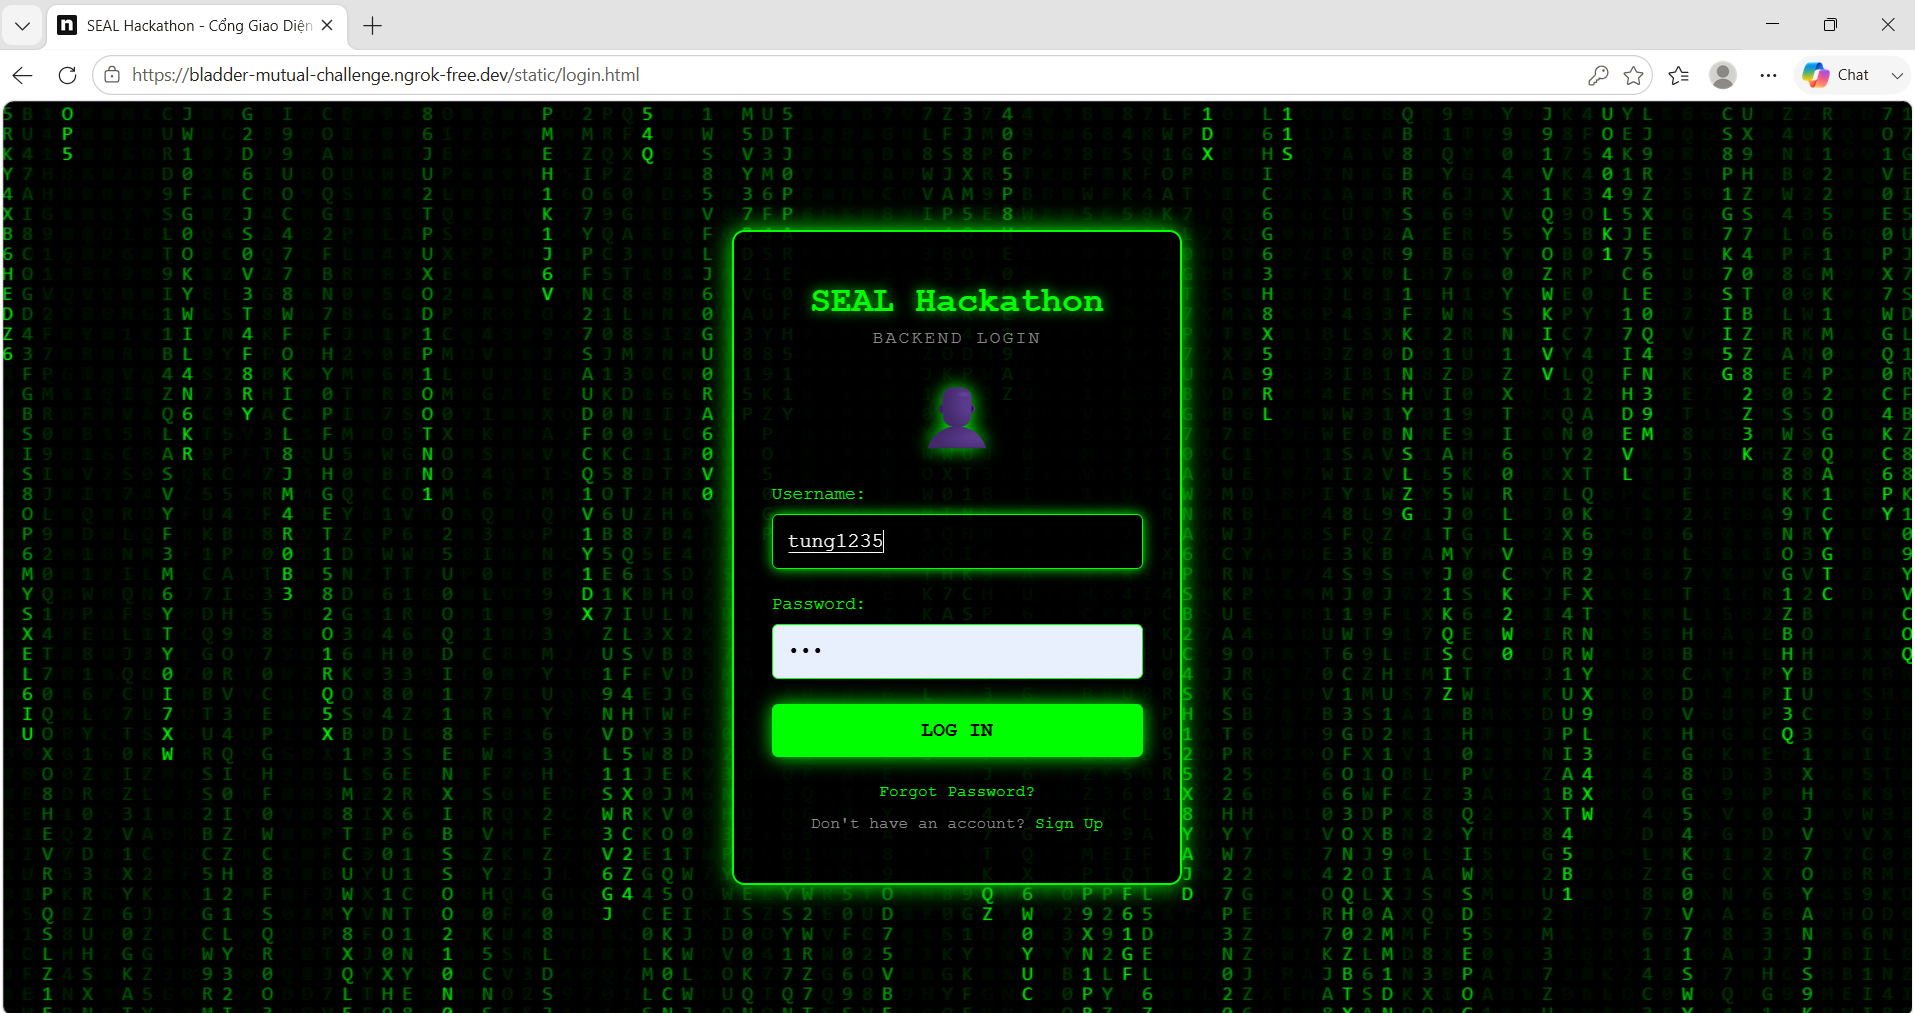
\includegraphics[width=0.82\textwidth]{images/register_success.png}
	\caption{Kết quả kiểm thử TC-REG-01}
	\label{fig:register-success}
\end{figure}

Kết quả kiểm thử cho thấy hệ thống đã xử lý chính xác dữ liệu hợp lệ, tài khoản mới được tạo thành công và lưu vào cơ sở dữ liệu.

%%%%%%%%%%%%%%%%%%%%%%%%%%%%%%%%%%%%%%%%%%%%%%%%%%%%%%%%%%%%%%%%%%%%%%%%%%%%%%
\subsection{TC-REG-02: Đăng ký với Username đã tồn tại}

\begin{table}[H]
	\centering
	\caption{Test Case TC-REG-02}
	\label{tab:tc-reg02}
	\renewcommand{\arraystretch}{1.3}
	
	\begin{tabular}{|p{4cm}|p{10cm}|}
		\hline
		\textbf{Thuộc tính} & \textbf{Nội dung} \\ \hline
		
		Test ID
		&
		TC-REG-02
		\\ \hline
		
		Chức năng
		&
		Đăng ký tài khoản
		\\ \hline
		
		Mục tiêu
		&
		Kiểm tra hệ thống phát hiện Username đã tồn tại.
		\\ \hline
		
		Điều kiện tiên quyết
		&
		Username tung123 đã tồn tại trong cơ sở dữ liệu.
		\\ \hline
		
		Dữ liệu đầu vào
		&
		Username: tung123
		
		Email: camxuan94@gmail.com
		\\ \hline
		
		Các bước thực hiện
		&
		1. Nhập Username đã tồn tại.
		
		2. Nhập Email mới.
		
		3. Nhấn Register.
		\\ \hline
		
		Kết quả mong đợi
		&
		Hệ thống không tạo tài khoản và hiển thị thông báo lỗi.
		\\ \hline
		
		Kết quả thực tế
		&
		Hệ thống hiển thị thông báo:
		
		"Đăng ký thất bại: Username hoặc Email đã được sử dụng!"
		\\ \hline
		
		Trạng thái
		&
		\textbf{PASS}
		\\ \hline
		
	\end{tabular}
\end{table}

\begin{figure}[H]
	\centering
	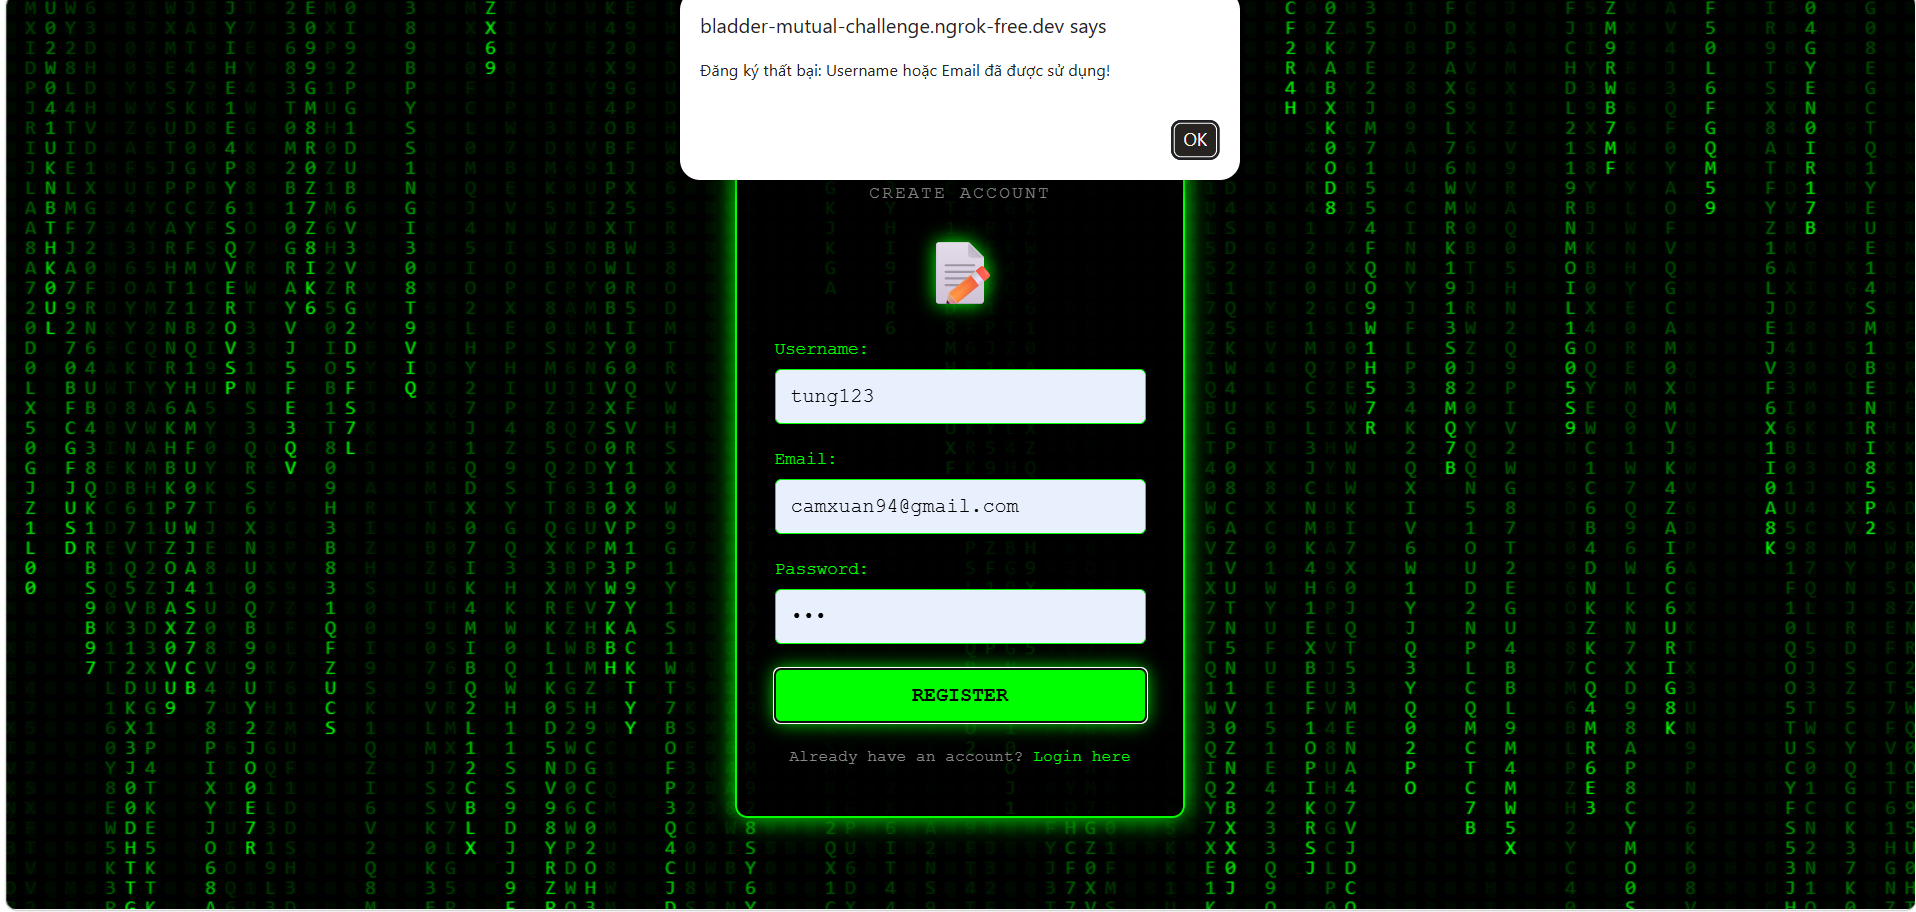
\includegraphics[width=0.82\textwidth]{images/register_duplicate_username.png}
	\caption{Kết quả kiểm thử TC-REG-02}
	\label{fig:duplicate-username}
\end{figure}

Qua quá trình kiểm thử, hệ thống đã ngăn chặn việc tạo trùng Username và đảm bảo tính toàn vẹn của dữ liệu người dùng.

%%%%%%%%%%%%%%%%%%%%%%%%%%%%%%%%%%%%%%%%%%%%%%%%%%%%%%%%%%%%%%%%%%%%%%%%%%%%%%
\subsection{TC-REG-03: Đăng ký với Email đã tồn tại}

\begin{table}[H]
	\centering
	\caption{Test Case TC-REG-03}
	\label{tab:tc-reg03}
	\renewcommand{\arraystretch}{1.3}
	
	\begin{tabular}{|p{4cm}|p{10cm}|}
		\hline
		\textbf{Thuộc tính} & \textbf{Nội dung} \\ \hline
		
		Test ID
		&
		TC-REG-03
		\\ \hline
		
		Chức năng
		&
		Đăng ký tài khoản
		\\ \hline
		
		Mục tiêu
		&
		Kiểm tra hệ thống phát hiện Email đã tồn tại.
		\\ \hline
		
		Điều kiện tiên quyết
		&
		Email camxuan94@gmail.com đã tồn tại trong cơ sở dữ liệu.
		\\ \hline
		
		Dữ liệu đầu vào
		&
		Username: tung1235
		
		Email: camxuan94@gmail.com
		\\ \hline
		
		Các bước thực hiện
		&
		1. Nhập Username mới.
		
		2. Nhập Email đã tồn tại.
		
		3. Nhấn Register.
		\\ \hline
		
		Kết quả mong đợi
		&
		Hệ thống từ chối tạo tài khoản và hiển thị thông báo lỗi.
		\\ \hline
		
		Kết quả thực tế
		&
		Hệ thống hiển thị thông báo:
		
		"Đăng ký thất bại: Username hoặc Email đã được sử dụng!"
		\\ \hline
		
		Trạng thái
		&
		\textbf{PASS}
		\\ \hline
		
	\end{tabular}
\end{table}

\begin{figure}[H]
	\centering
	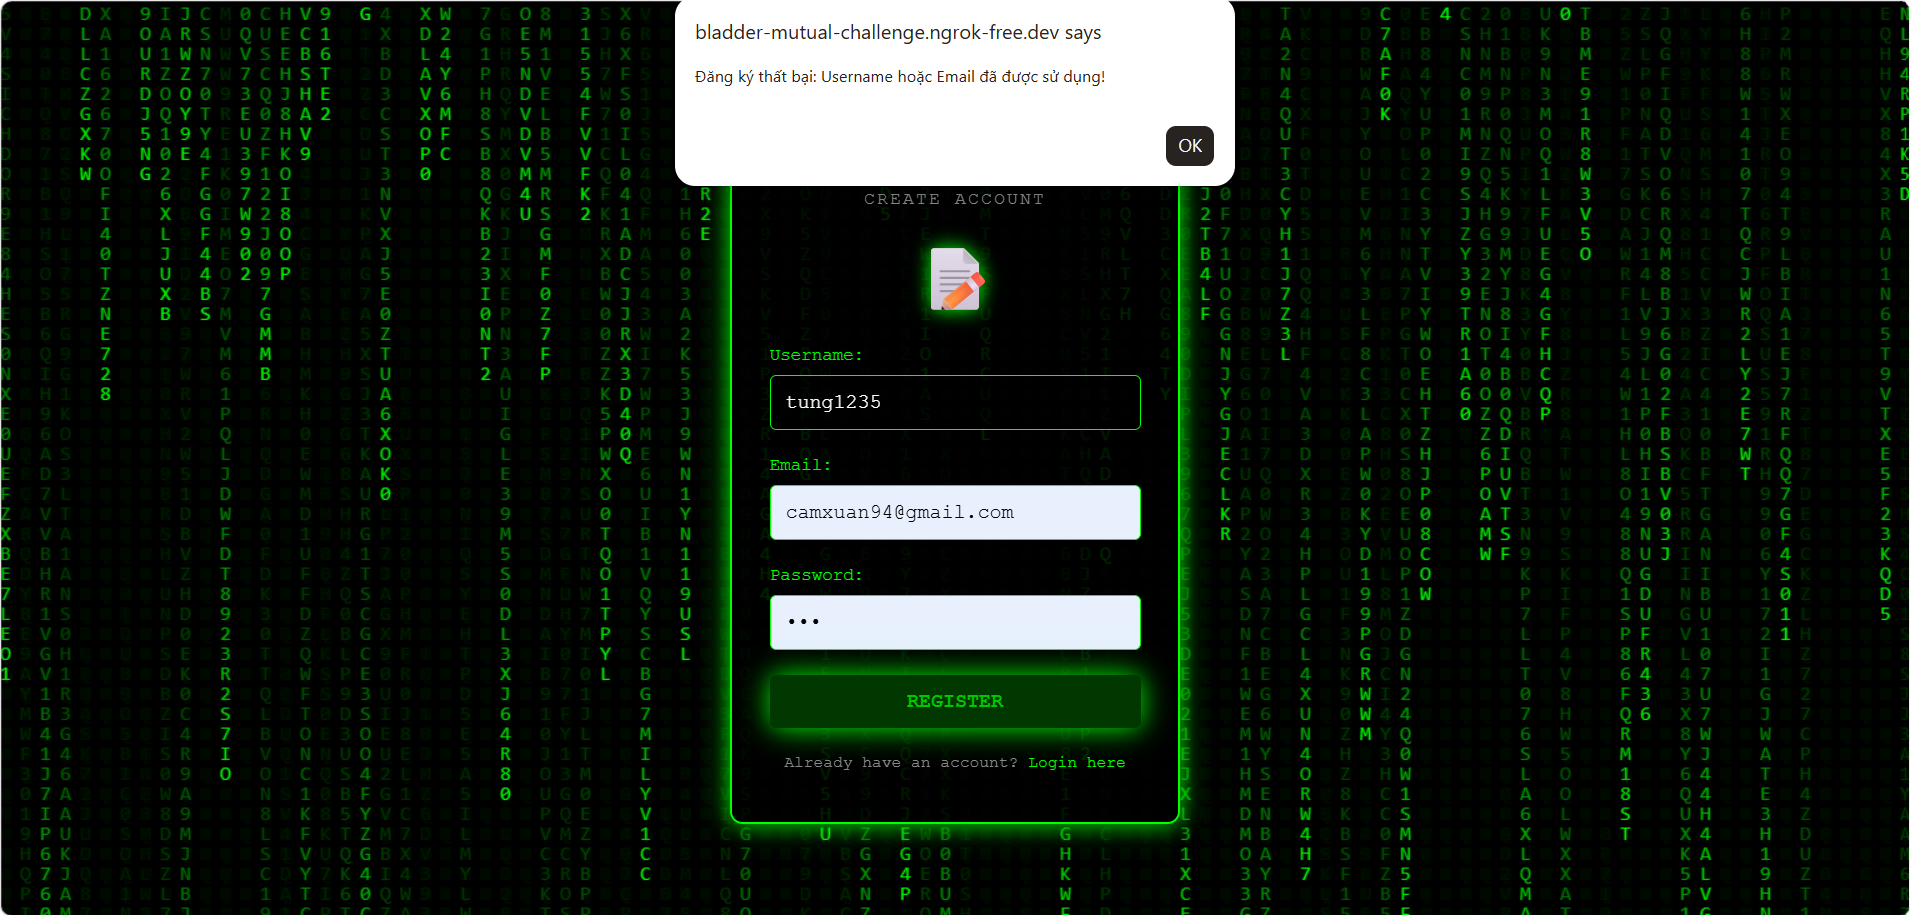
\includegraphics[width=0.82\textwidth]{images/register_duplicate_email.png}
	\caption{Kết quả kiểm thử TC-REG-03}
	\label{fig:duplicate-email}
\end{figure}

Kết quả kiểm thử cho thấy hệ thống đã kiểm tra thành công tính duy nhất của địa chỉ Email trước khi tạo tài khoản mới, góp phần hạn chế dữ liệu trùng lặp trong cơ sở dữ liệu.
%%%%%%%%%%%%%%%%%%%%%%%%%%%%%%%%%%%%%%%%%%%%%%%%%%%%%%%%%%%%%%%%%%%%%%%%%%%%%%
\section{Kiểm thử chức năng đăng nhập}
%%%%%%%%%%%%%%%%%%%%%%%%%%%%%%%%%%%%%%%%%%%%%%%%%%%%%%%%%%%%%%%%%%%%%%%%%%%%%%

Chức năng đăng nhập cho phép người dùng truy cập vào hệ thống bằng tài khoản đã được đăng ký trước đó. Đây là chức năng quan trọng nhằm xác thực danh tính người dùng, phân quyền truy cập và bảo vệ dữ liệu của hệ thống.

Nhóm tiến hành kiểm thử các trường hợp đăng nhập hợp lệ và không hợp lệ nhằm đánh giá khả năng xác thực của hệ thống cũng như cơ chế xử lý lỗi khi người dùng nhập sai thông tin.

%%%%%%%%%%%%%%%%%%%%%%%%%%%%%%%%%%%%%%%%%%%%%%%%%%%%%%%%%%%%%%%%%%%%%%%%%%%%%%
\subsection{TC-LOGIN-01: Đăng nhập thành công}

\begin{table}[H]
	\centering
	\caption{Test Case TC-LOGIN-01}
	\label{tab:tc-login01}
	\renewcommand{\arraystretch}{1.3}
	
	\begin{tabular}{|p{4cm}|p{10cm}|}
		\hline
		\textbf{Thuộc tính} & \textbf{Nội dung} \\ \hline
		
		Test ID &
		TC-LOGIN-01
		\\ \hline
		
		Chức năng &
		Đăng nhập hệ thống
		\\ \hline
		
		Mục tiêu &
		Kiểm tra hệ thống cho phép người dùng đăng nhập bằng tài khoản hợp lệ.
		\\ \hline
		
		Điều kiện tiên quyết &
		Người dùng đã có tài khoản trong cơ sở dữ liệu.
		\\ \hline
		
		Dữ liệu đầu vào &
		Username: tung123
		
		Password: 123
		\\ \hline
		
		Các bước thực hiện &
		1. Truy cập trang Login.
		
		2. Nhập Username.
		
		3. Nhập Password.
		
		4. Nhấn nút Login.
		\\ \hline
		
		Kết quả mong đợi &
		Hệ thống xác thực thành công và chuyển người dùng đến Dashboard.
		\\ \hline
		
		Kết quả thực tế &
		Đăng nhập thành công và hiển thị giao diện Dashboard.
		\\ \hline
		
		Trạng thái &
		\textbf{PASS}
		\\ \hline
		
	\end{tabular}
\end{table}

\begin{figure}[H]
	\centering
	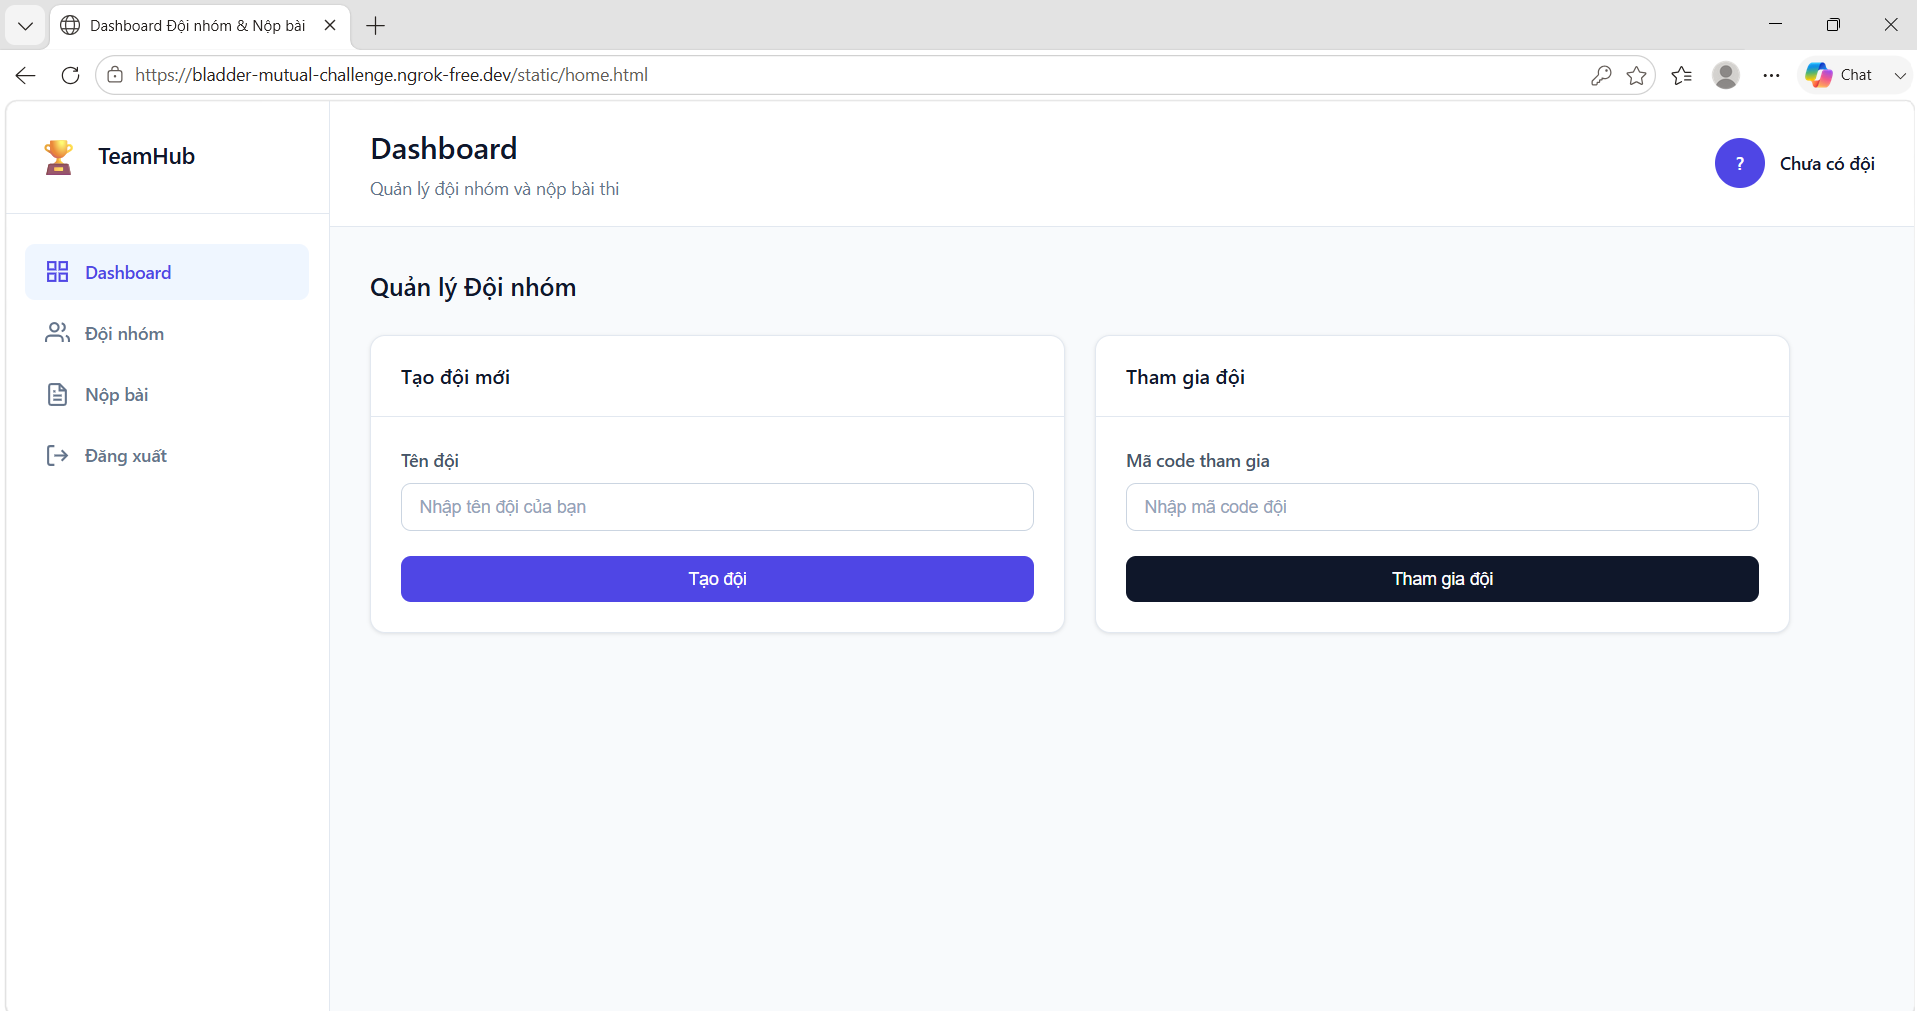
\includegraphics[width=0.82\textwidth]{images/login_success.png}
	\caption{Kết quả kiểm thử TC-LOGIN-01}
	\label{fig:login-success}
\end{figure}

Kết quả kiểm thử cho thấy hệ thống xác thực thành công tài khoản hợp lệ và chuyển người dùng đến giao diện Dashboard đúng theo yêu cầu thiết kế.

%%%%%%%%%%%%%%%%%%%%%%%%%%%%%%%%%%%%%%%%%%%%%%%%%%%%%%%%%%%%%%%%%%%%%%%%%%%%%%
\subsection{TC-LOGIN-02: Đăng nhập với mật khẩu không chính xác}

\begin{table}[H]
	\centering
	\caption{Test Case TC-LOGIN-02}
	\label{tab:tc-login02}
	\renewcommand{\arraystretch}{1.3}
	
	\begin{tabular}{|p{4cm}|p{10cm}|}
		\hline
		\textbf{Thuộc tính} & \textbf{Nội dung} \\ \hline
		
		Test ID &
		TC-LOGIN-02
		\\ \hline
		
		Chức năng &
		Đăng nhập hệ thống
		\\ \hline
		
		Mục tiêu &
		Kiểm tra khả năng xử lý khi người dùng nhập sai mật khẩu.
		\\ \hline
		
		Điều kiện tiên quyết &
		Tài khoản đã tồn tại trong cơ sở dữ liệu.
		\\ \hline
		
		Dữ liệu đầu vào &
		Username: tung123
		
		Password: 123456
		\\ \hline
		
		Các bước thực hiện &
		1. Truy cập trang Login.
		
		2. Nhập Username hợp lệ.
		
		3. Nhập Password sai.
		
		4. Nhấn Login.
		\\ \hline
		
		Kết quả mong đợi &
		Hệ thống từ chối đăng nhập và hiển thị thông báo lỗi.
		\\ \hline
		
		Kết quả thực tế &
		Hệ thống không cho phép đăng nhập và hiển thị thông báo sai thông tin đăng nhập.
		\\ \hline
		
		Trạng thái &
		\textbf{PASS}
		\\ \hline
		
	\end{tabular}
\end{table}

\begin{figure}[H]
	\centering
	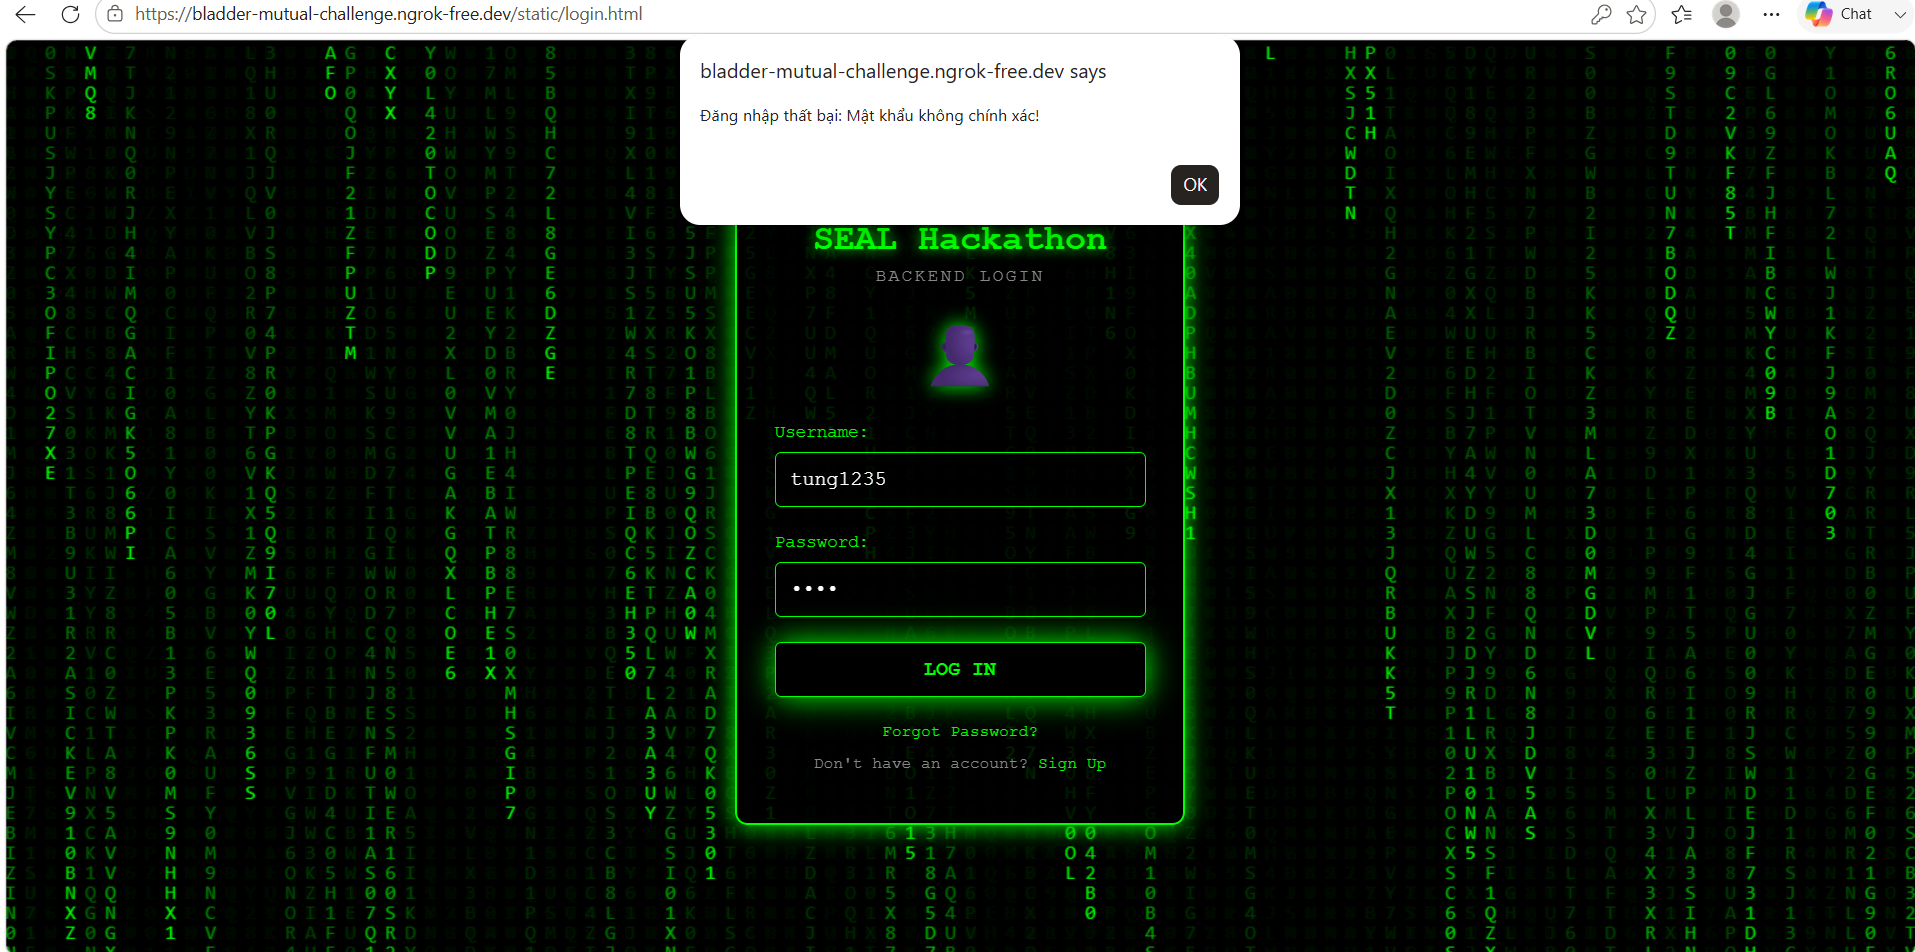
\includegraphics[width=0.82\textwidth]{images/login_failed.png}
	\caption{Kết quả kiểm thử TC-LOGIN-02}
	\label{fig:login-failed}
\end{figure}

Kết quả kiểm thử cho thấy hệ thống đã từ chối truy cập đối với tài khoản có mật khẩu không hợp lệ, góp phần đảm bảo tính an toàn cho hệ thống.
%%%%%%%%%%%%%%%%%%%%%%%%%%%%%%%%%%%%%%%%%%%%%%%%%%%%%%%%%%%%%%%%%%%%%%%%%%%%%%
\section{Kiểm thử chức năng quản lý đội nhóm}
%%%%%%%%%%%%%%%%%%%%%%%%%%%%%%%%%%%%%%%%%%%%%%%%%%%%%%%%%%%%%%%%%%%%%%%%%%%%%%

Chức năng quản lý đội nhóm là chức năng trung tâm của hệ thống SEAL Hackathon Management System. Chức năng này cho phép người dùng tạo đội mới, tham gia đội thông qua mã mời, xem thông tin đội và quản lý thành viên theo quyền hạn của từng người dùng.

Trong quá trình kiểm thử, nhóm tiến hành đánh giá các chức năng chính bao gồm tạo đội, hiển thị thông tin đội và khả năng xử lý giao diện khi người dùng chưa tham gia đội.

%%%%%%%%%%%%%%%%%%%%%%%%%%%%%%%%%%%%%%%%%%%%%%%%%%%%%%%%%%%%%%%%%%%%%%%%%%%%%%
\subsection{TC-TEAM-01: Hiển thị Dashboard khi chưa có đội}

\begin{table}[H]
	\centering
	\caption{Test Case TC-TEAM-01}
	\label{tab:tc-team01}
	\renewcommand{\arraystretch}{1.3}
	
	\begin{tabular}{|p{4cm}|p{10cm}|}
		\hline
		\textbf{Thuộc tính} & \textbf{Nội dung} \\ \hline
		
		Test ID &
		TC-TEAM-01
		\\ \hline
		
		Chức năng &
		Dashboard
		\\ \hline
		
		Mục tiêu &
		Kiểm tra giao diện Dashboard khi người dùng chưa thuộc đội nào.
		\\ \hline
		
		Điều kiện tiên quyết &
		Người dùng đã đăng nhập thành công và chưa tạo hoặc tham gia đội.
		\\ \hline
		
		Các bước thực hiện &
		1. Đăng nhập vào hệ thống.
		
		2. Truy cập Dashboard.
		\\ \hline
		
		Kết quả mong đợi &
		Hiển thị giao diện tạo đội và tham gia đội.
		
		Không hiển thị danh sách thành viên.
		\\ \hline
		
		Kết quả thực tế &
		Dashboard hiển thị đúng trạng thái "Chưa có đội", cho phép tạo hoặc tham gia đội.
		\\ \hline
		
		Trạng thái &
		\textbf{PASS}
		\\ \hline
		
	\end{tabular}
	
\end{table}

\begin{figure}[H]
	\centering
	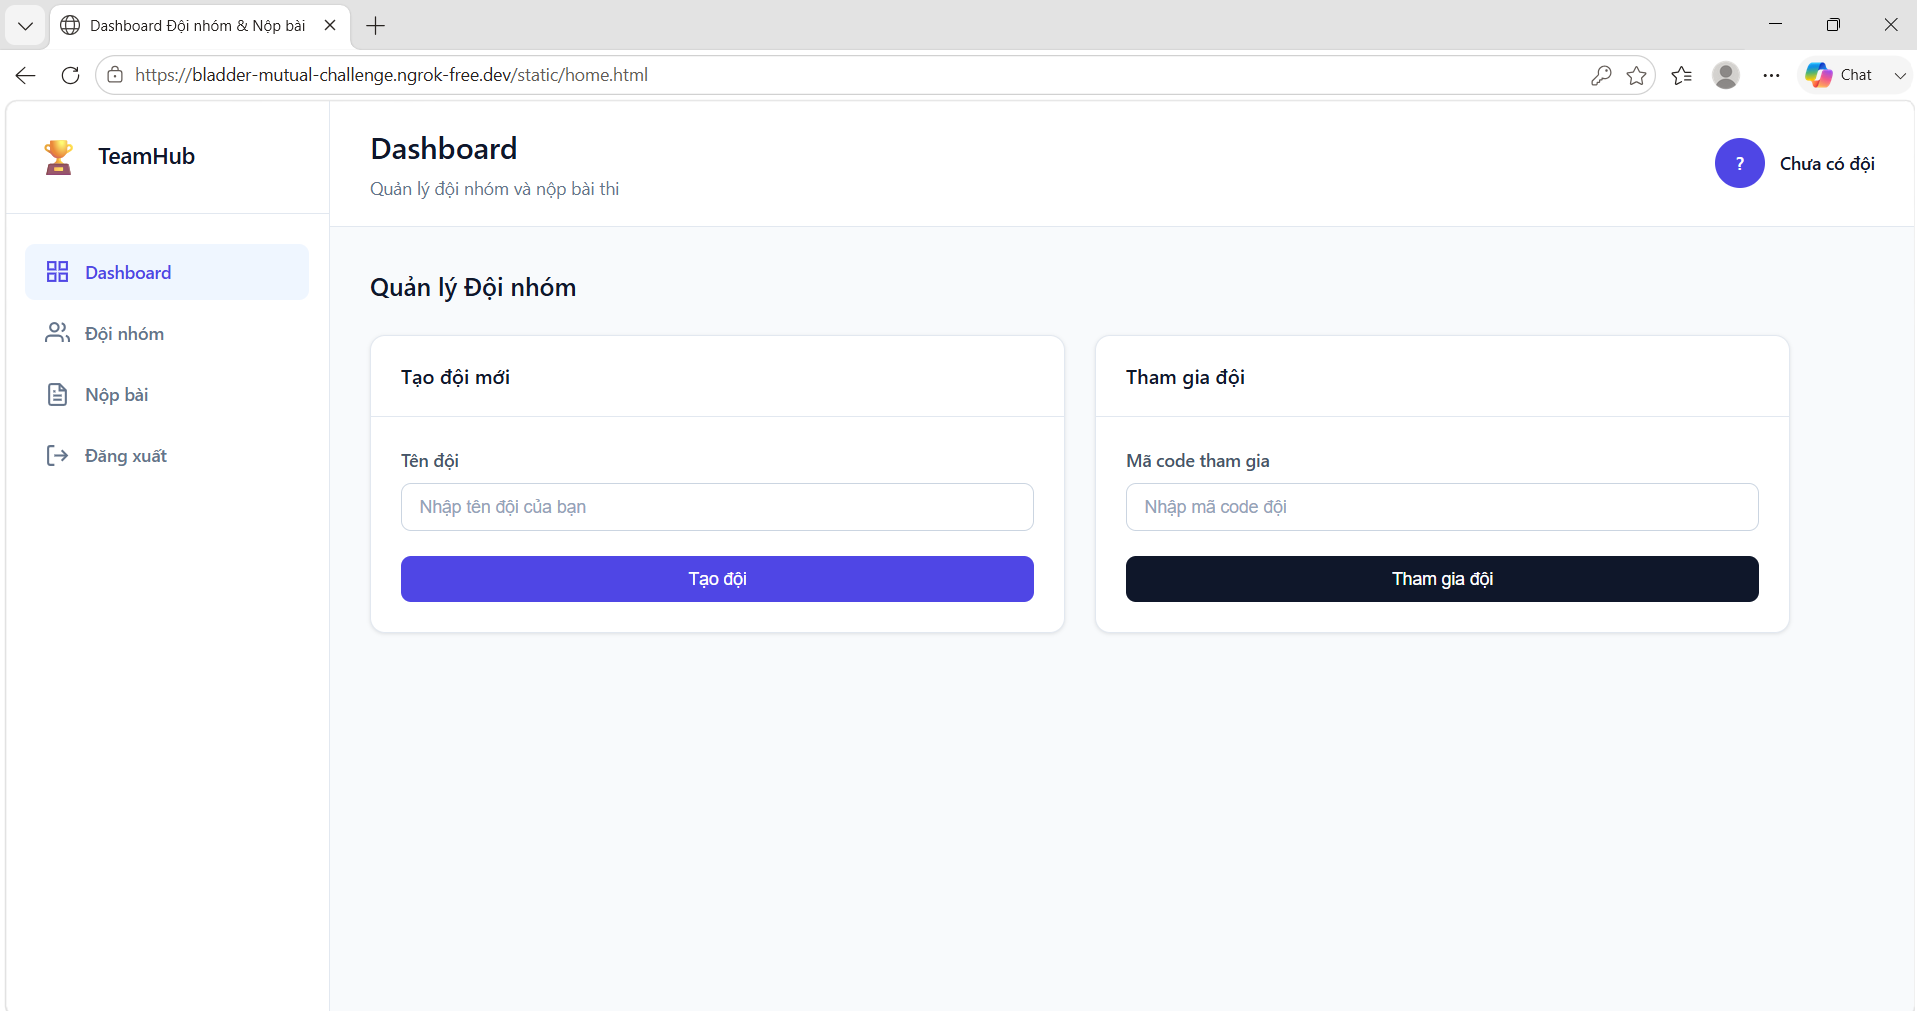
\includegraphics[width=0.82\textwidth]{images/dashboard_no_team.png}
	\caption{Kết quả kiểm thử TC-TEAM-01}
	\label{fig:dashboard-noteam}
\end{figure}

Hệ thống hiển thị chính xác giao diện dành cho người dùng chưa thuộc đội nào và ẩn các thông tin quản lý thành viên.

%%%%%%%%%%%%%%%%%%%%%%%%%%%%%%%%%%%%%%%%%%%%%%%%%%%%%%%%%%%%%%%%%%%%%%%%%%%%%%
\subsection{TC-TEAM-02: Tạo đội thành công}

\begin{table}[H]
	\centering
	\caption{Test Case TC-TEAM-02}
	\label{tab:tc-team02}
	\renewcommand{\arraystretch}{1.3}
	
	\begin{tabular}{|p{4cm}|p{10cm}|}
		\hline
		\textbf{Thuộc tính} & \textbf{Nội dung} \\ \hline
		
		Test ID &
		TC-TEAM-02
		\\ \hline
		
		Chức năng &
		Tạo đội
		\\ \hline
		
		Mục tiêu &
		Kiểm tra khả năng tạo đội mới.
		\\ \hline
		
		Điều kiện tiên quyết &
		Người dùng chưa thuộc bất kỳ đội nào.
		\\ \hline
		
		Dữ liệu đầu vào &
		Tên đội: AI BOT
		\\ \hline
		
		Các bước thực hiện &
		1. Nhập tên đội.
		
		2. Nhấn nút Tạo đội.
		\\ \hline
		
		Kết quả mong đợi &
		Hệ thống tạo đội thành công và hiển thị thông báo xác nhận.
		\\ \hline
		
		Kết quả thực tế &
		Đội được tạo thành công và hiển thị thông báo "Tạo đội thành công!".
		\\ \hline
		
		Trạng thái &
		\textbf{PASS}
		\\ \hline
		
	\end{tabular}
	
\end{table}

\begin{figure}[H]
	\centering
	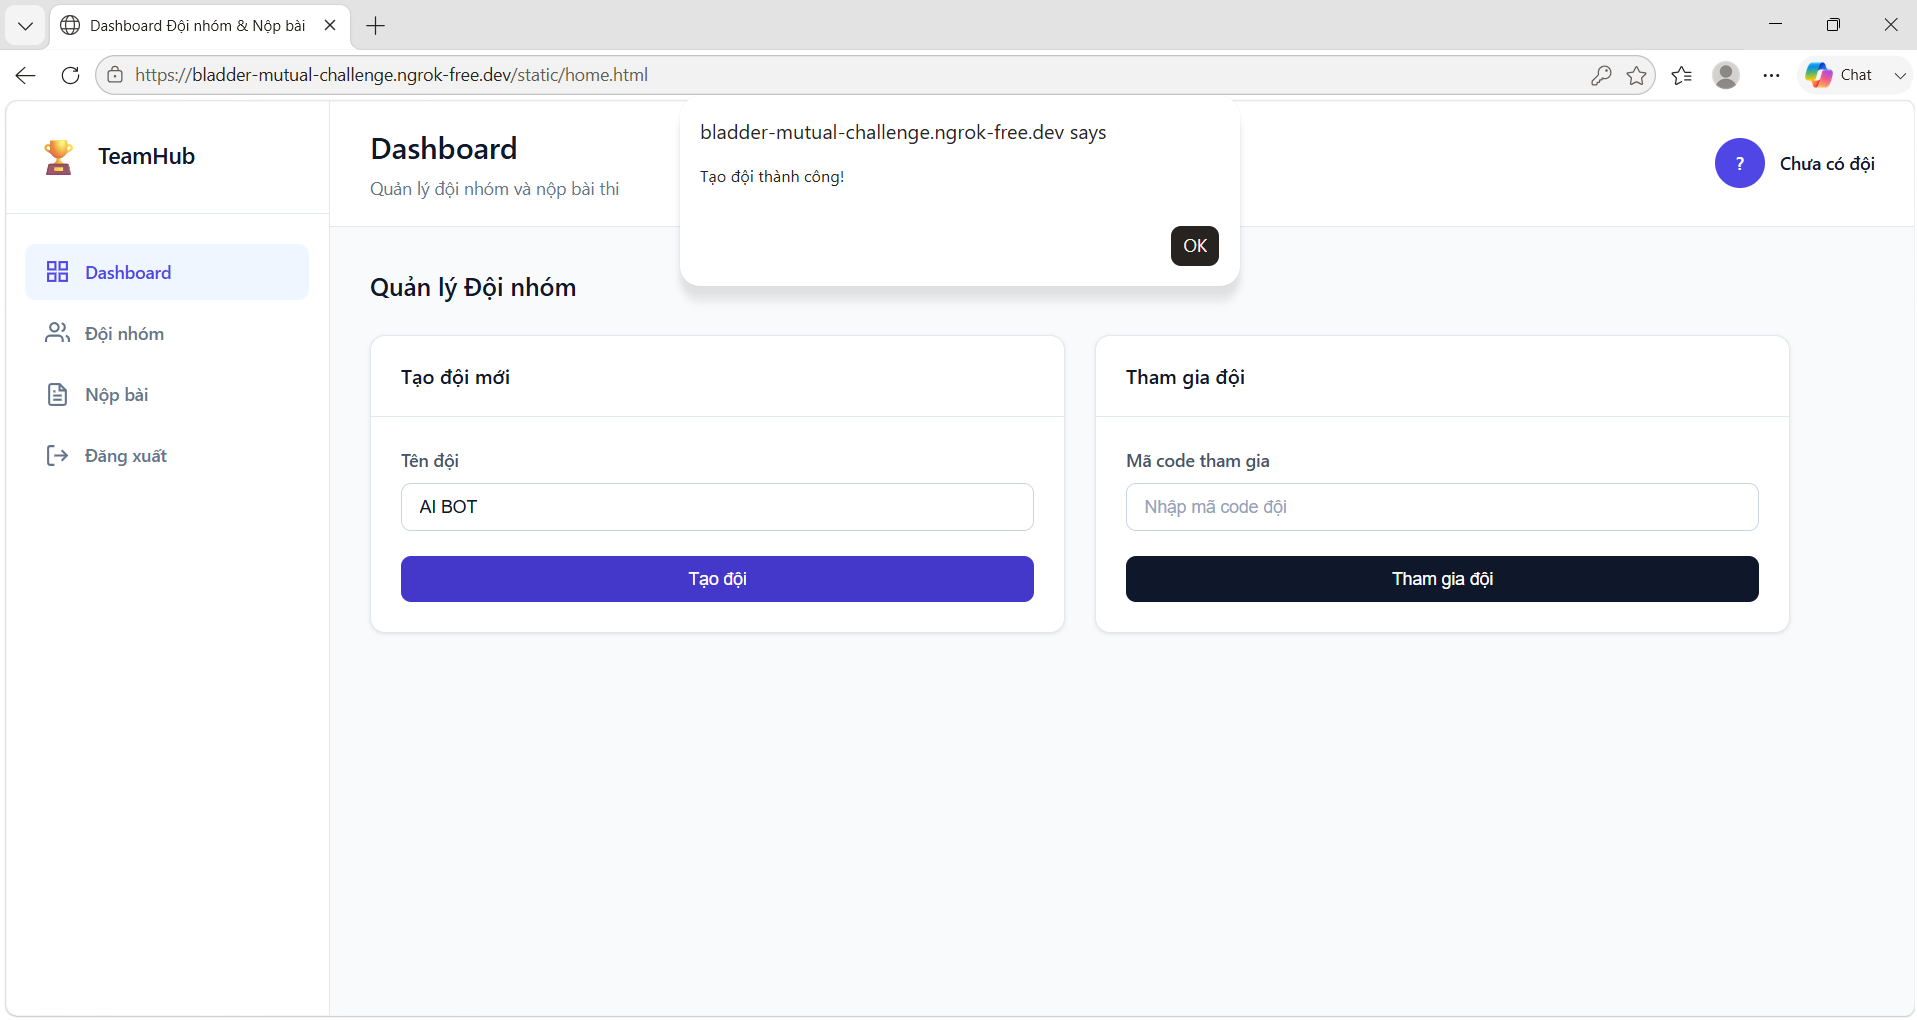
\includegraphics[width=0.82\textwidth]{images/create_team_success.png}
	\caption{Kết quả kiểm thử TC-TEAM-02}
	\label{fig:create-team}
\end{figure}

Kết quả kiểm thử cho thấy hệ thống tạo đội thành công và phản hồi đúng cho người dùng.

%%%%%%%%%%%%%%%%%%%%%%%%%%%%%%%%%%%%%%%%%%%%%%%%%%%%%%%%%%%%%%%%%%%%%%%%%%%%%%
\subsection{TC-TEAM-03: Hiển thị thông tin đội sau khi tạo}

\begin{table}[H]
	\centering
	\caption{Test Case TC-TEAM-03}
	\label{tab:tc-team03}
	\renewcommand{\arraystretch}{1.3}
	
	\begin{tabular}{|p{4cm}|p{10cm}|}
		\hline
		\textbf{Thuộc tính} & \textbf{Nội dung} \\ \hline
		
		Test ID &
		TC-TEAM-03
		\\ \hline
		
		Chức năng &
		Thông tin đội
		\\ \hline
		
		Mục tiêu &
		Kiểm tra hệ thống hiển thị đầy đủ thông tin sau khi tạo đội.
		\\ \hline
		
		Điều kiện tiên quyết &
		Người dùng đã tạo đội thành công.
		\\ \hline
		
		Các bước thực hiện &
		1. Tạo đội thành công.
		
		2. Quan sát Dashboard.
		\\ \hline
		
		Kết quả mong đợi &
		Hiển thị:
		
		- Tên đội
		
		- Mã mời
		
		- Vai trò Trưởng đội
		
		- Nút Giải tán đội
		\\ \hline
		
		Kết quả thực tế &
		Toàn bộ thông tin đội được hiển thị đúng theo thiết kế.
		\\ \hline
		
		Trạng thái &
		\textbf{PASS}
		\\ \hline
		
	\end{tabular}
	
\end{table}

\begin{figure}[H]
	\centering
	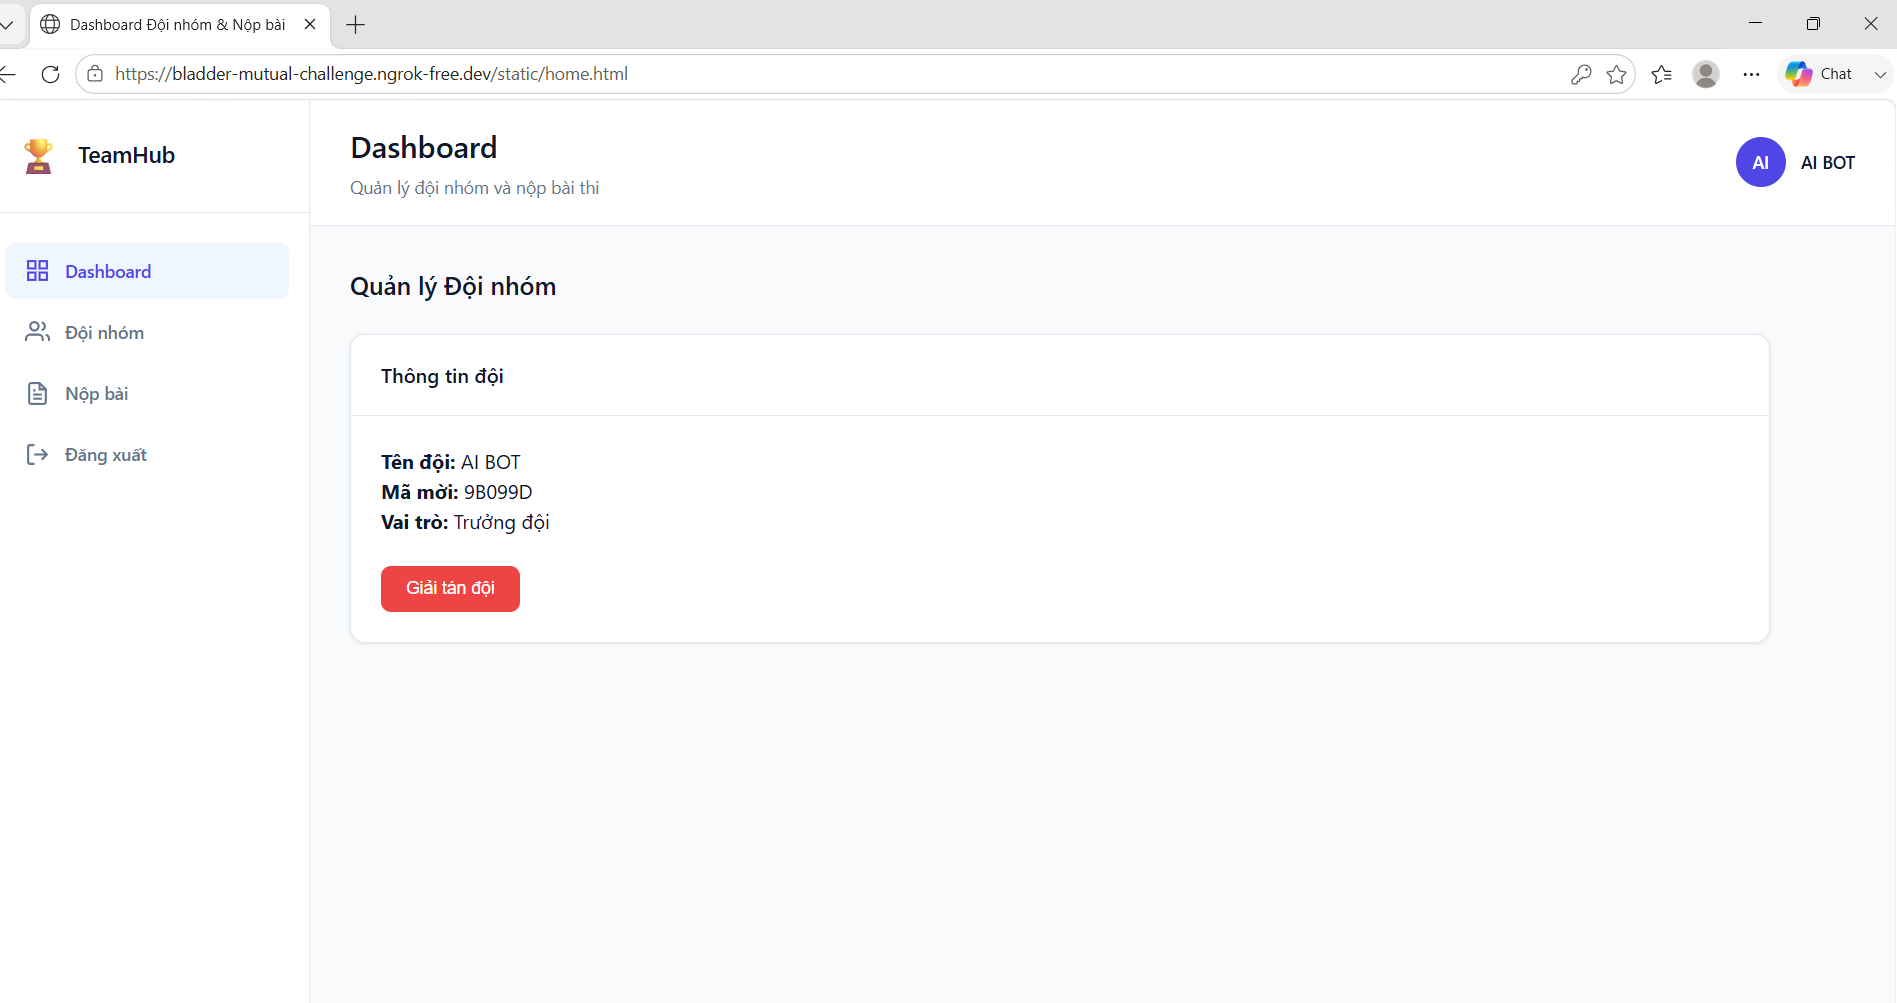
\includegraphics[width=0.82\textwidth]{images/dashboard_team_info.png}
	\caption{Kết quả kiểm thử TC-TEAM-03}
	\label{fig:team-info}
\end{figure}

Sau khi tạo đội thành công, hệ thống tự động cập nhật giao diện Dashboard, hiển thị đầy đủ thông tin đội và quyền của Trưởng đội.
%%%%%%%%%%%%%%%%%%%%%%%%%%%%%%%%%%%%%%%%%%%%%%%%%%%%%%%%%%%%%%%%%%%%%%%%%%%%%%
\section{Kiểm thử chức năng quản lý thành viên}
%%%%%%%%%%%%%%%%%%%%%%%%%%%%%%%%%%%%%%%%%%%%%%%%%%%%%%%%%%%%%%%%%%%%%%%%%%%%%%

Sau khi đội được tạo thành công, hệ thống cho phép người dùng khác gửi yêu cầu tham gia thông qua mã mời. Trưởng đội có quyền xem danh sách chờ, phê duyệt hoặc từ chối yêu cầu tham gia, đồng thời có thể loại thành viên khỏi đội khi cần thiết.

Các chức năng này được kiểm thử nhằm đảm bảo việc quản lý thành viên diễn ra đúng theo quy tắc nghiệp vụ đã thiết kế.

%%%%%%%%%%%%%%%%%%%%%%%%%%%%%%%%%%%%%%%%%%%%%%%%%%%%%%%%%%%%%%%%%%%%%%%%%%%%%%
\subsection{TC-MEMBER-01: Tham gia đội thành công}

\begin{table}[H]
	\centering
	\caption{Test Case TC-MEMBER-01}
	\label{tab:tc-member01}
	\renewcommand{\arraystretch}{1.3}
	
	\begin{tabular}{|p{4cm}|p{10cm}|}
		\hline
		\textbf{Thuộc tính} & \textbf{Nội dung} \\ \hline
		
		Test ID &
		TC-MEMBER-01
		\\ \hline
		
		Chức năng &
		Tham gia đội
		\\ \hline
		
		Mục tiêu &
		Kiểm tra người dùng gửi yêu cầu tham gia đội bằng mã mời hợp lệ.
		\\ \hline
		
		Điều kiện tiên quyết &
		Đã tồn tại một đội và người dùng chưa thuộc đội nào.
		\\ \hline
		
		Dữ liệu đầu vào &
		Mã mời hợp lệ.
		\\ \hline
		
		Các bước thực hiện &
		1. Đăng nhập.
		
		2. Chọn "Tham gia đội".
		
		3. Nhập mã mời.
		
		4. Nhấn nút Xác nhận.
		\\ \hline
		
		Kết quả mong đợi &
		Hệ thống gửi yêu cầu tham gia và thông báo thành công.
		\\ \hline
		
		Kết quả thực tế &
		Yêu cầu tham gia được ghi nhận thành công.
		\\ \hline
		
		Trạng thái &
		\textbf{PASS}
		\\ \hline
		
	\end{tabular}
\end{table}

\begin{figure}[H]
	\centering
	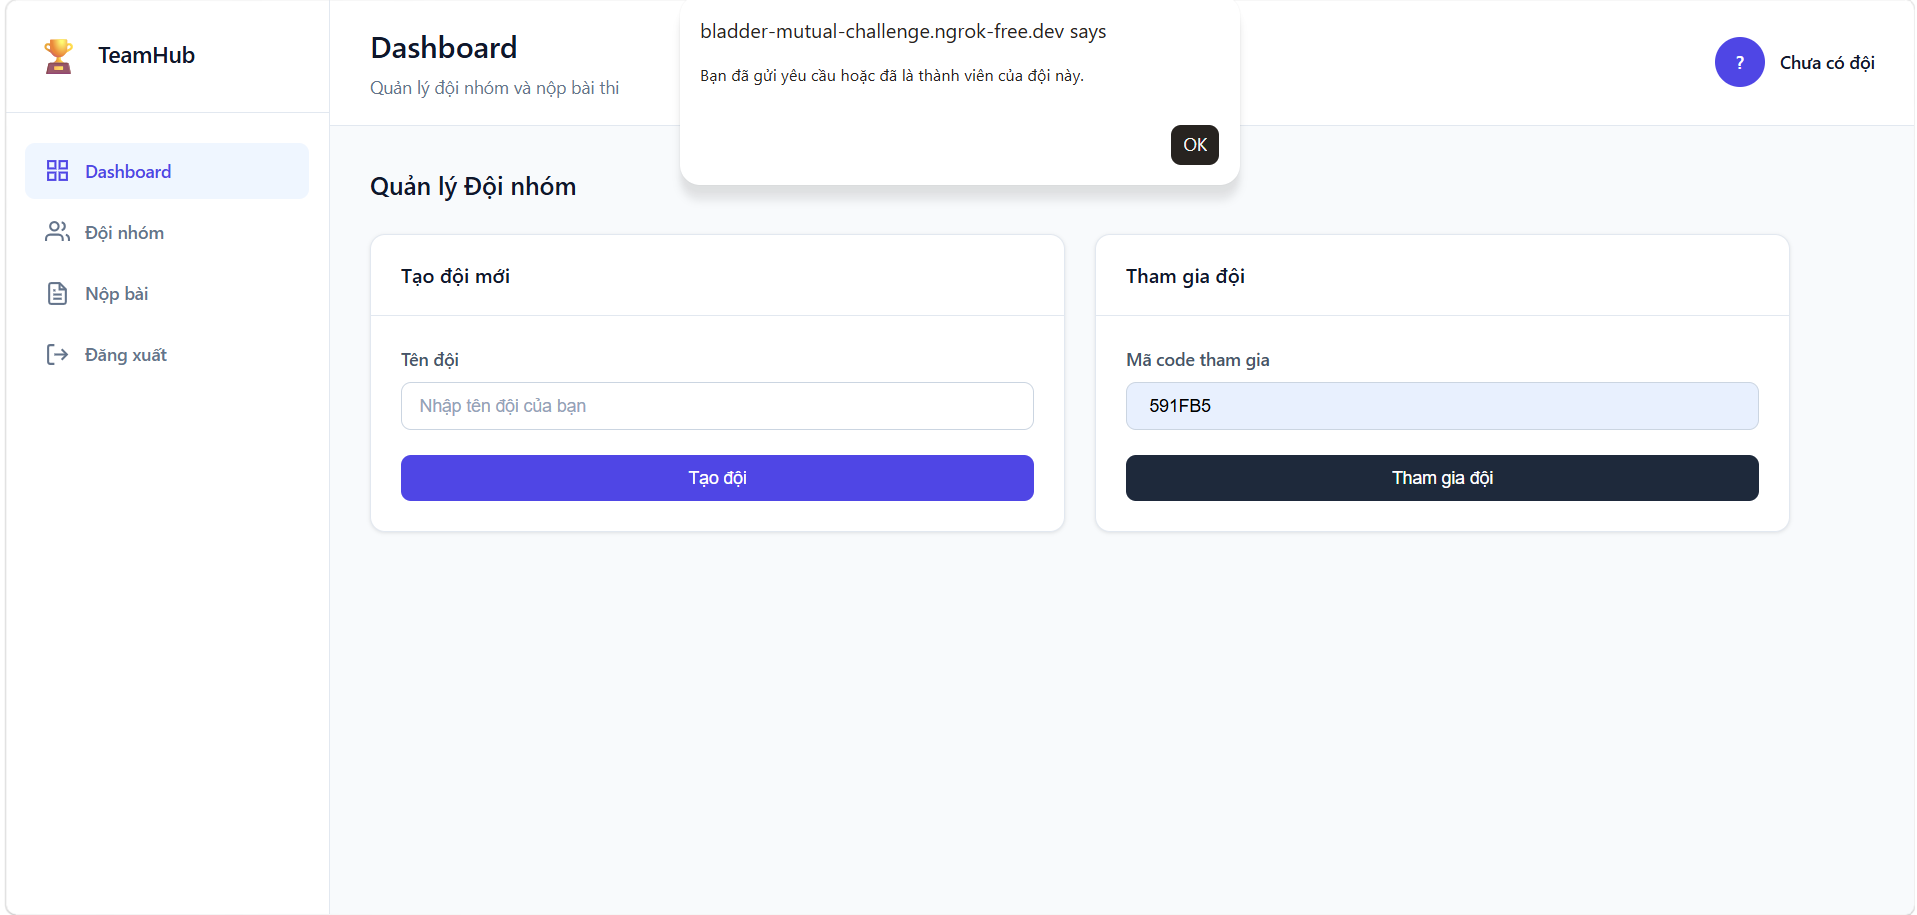
\includegraphics[width=0.82\textwidth]{images/join_team_success.png}
	\caption{Kiểm thử TC-MEMBER-01}
	\label{fig:join-team}
\end{figure}

%%%%%%%%%%%%%%%%%%%%%%%%%%%%%%%%%%%%%%%%%%%%%%%%%%%%%%%%%%%%%%%%%%%%%%%%%%%%%%
\subsection{TC-MEMBER-02: Mã mời không hợp lệ}

\begin{table}[H]
	\centering
	\caption{Test Case TC-MEMBER-02}
	\label{tab:tc-member02}
	\renewcommand{\arraystretch}{1.3}
	
	\begin{tabular}{|p{4cm}|p{10cm}|}
		\hline
		\textbf{Thuộc tính} & \textbf{Nội dung} \\ \hline
		
		Test ID &
		TC-MEMBER-02
		\\ \hline
		
		Chức năng &
		Tham gia đội
		\\ \hline
		
		Mục tiêu &
		Kiểm tra khả năng xử lý khi người dùng nhập sai mã đội.
		\\ \hline
		
		Điều kiện tiên quyết &
		Người dùng chưa thuộc đội.
		\\ \hline
		
		Dữ liệu đầu vào &
		ABCDE1
		\\ \hline
		
		Các bước thực hiện &
		Nhập mã đội không tồn tại rồi xác nhận.
		\\ \hline
		
		Kết quả mong đợi &
		Thông báo "Mã đội không hợp lệ."
		\\ \hline
		
		Kết quả thực tế &
		Hệ thống từ chối yêu cầu tham gia.
		\\ \hline
		
		Trạng thái &
		\textbf{PASS}
		\\ \hline
		
	\end{tabular}
\end{table}

\begin{figure}[H]
	\centering
	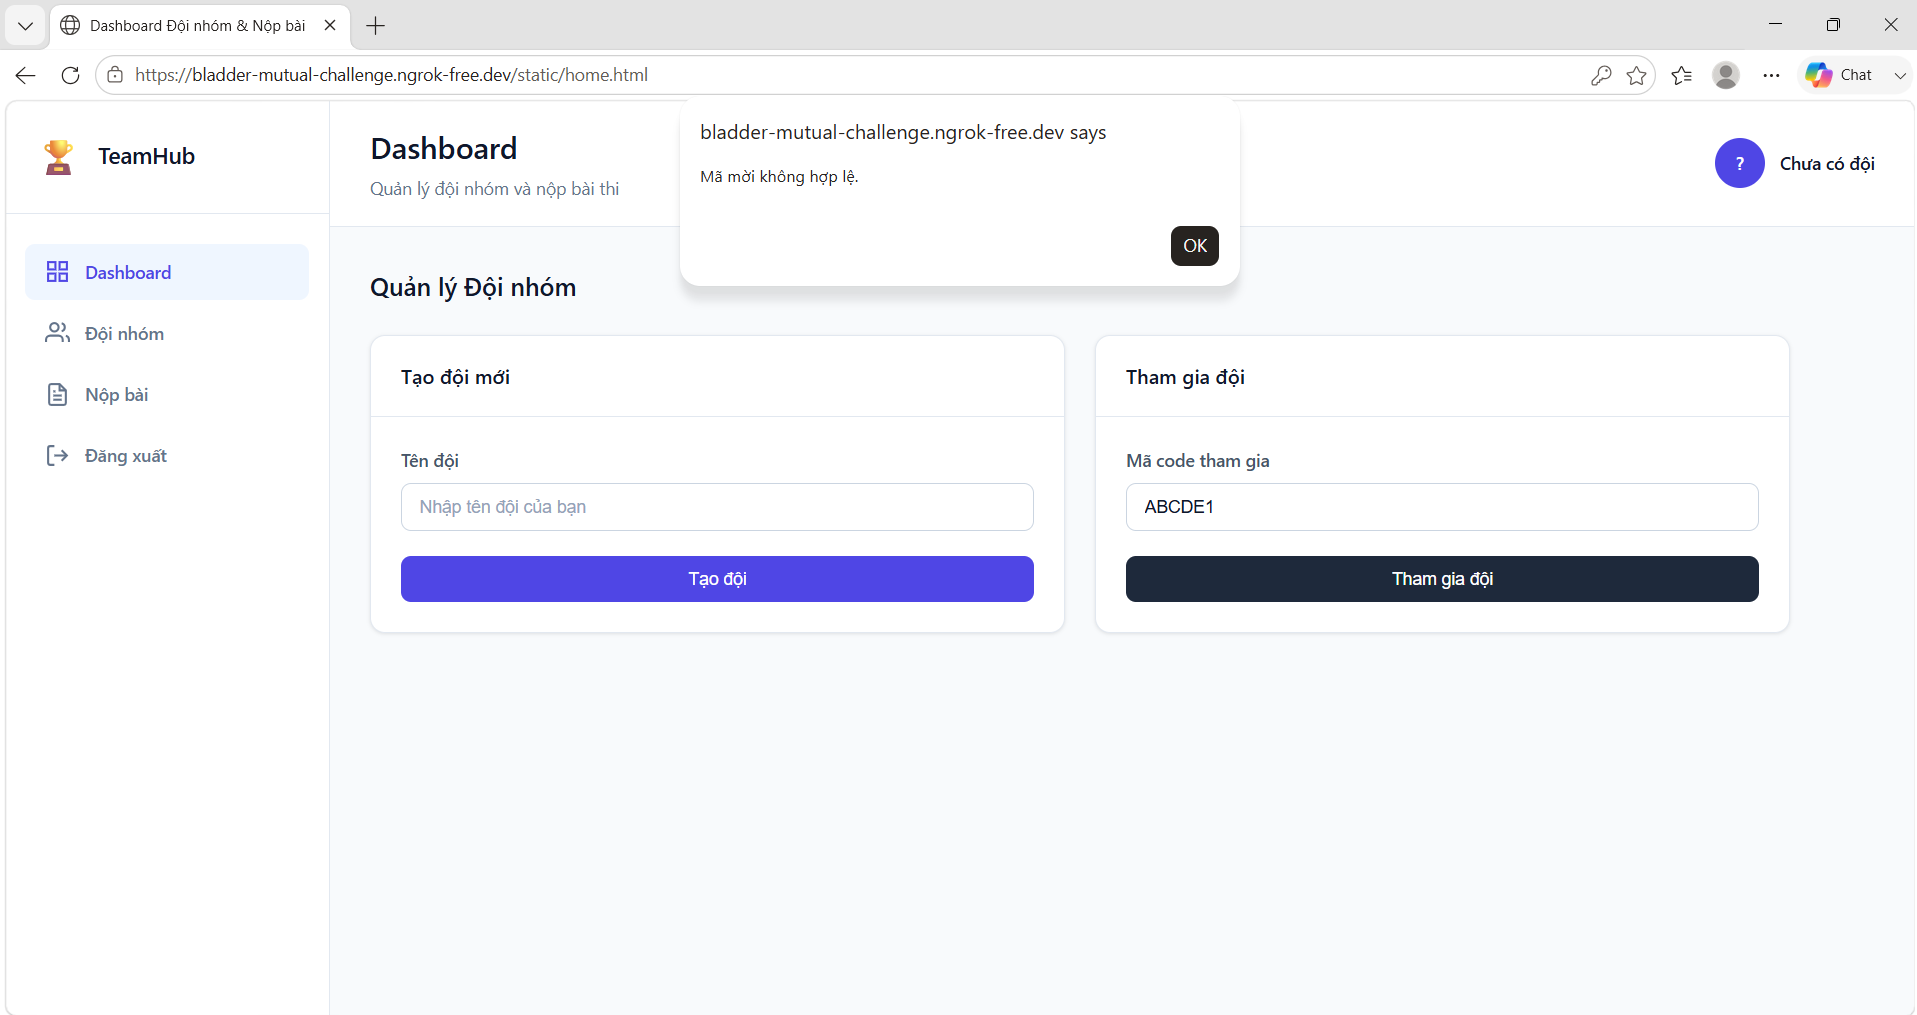
\includegraphics[width=0.82\textwidth]{images/join_team_failed.png}
	\caption{Kiểm thử TC-MEMBER-02}
	\label{fig:join-team-failed}
\end{figure}

%%%%%%%%%%%%%%%%%%%%%%%%%%%%%%%%%%%%%%%%%%%%%%%%%%%%%%%%%%%%%%%%%%%%%%%%%%%%%%
\subsection{TC-MEMBER-03: Trưởng đội phê duyệt thành viên}

\begin{table}[H]
	\centering
	\caption{Test Case TC-MEMBER-03}
	\label{tab:tc-member03}
	\renewcommand{\arraystretch}{1.3}
	
	\begin{tabular}{|p{4cm}|p{10cm}|}
		\hline
		\textbf{Thuộc tính} & \textbf{Nội dung} \\ \hline
		
		Test ID &
		TC-MEMBER-03
		\\ \hline
		
		Chức năng &
		Duyệt thành viên
		\\ \hline
		
		Mục tiêu &
		Kiểm tra Leader có thể duyệt thành viên.
		\\ \hline
		
		Điều kiện tiên quyết &
		Có ít nhất một yêu cầu đang chờ.
		\\ \hline
		
		Các bước thực hiện &
		Nhấn nút "Đồng ý".
		\\ \hline
		
		Kết quả mong đợi &
		Người dùng được chuyển sang danh sách thành viên chính thức.
		\\ \hline
		
		Kết quả thực tế &
		Thành viên xuất hiện trong danh sách đội.
		\\ \hline
		
		Trạng thái &
		\textbf{PASS}
		\\ \hline
		
	\end{tabular}
\end{table}

\begin{figure}[H]
	\centering
	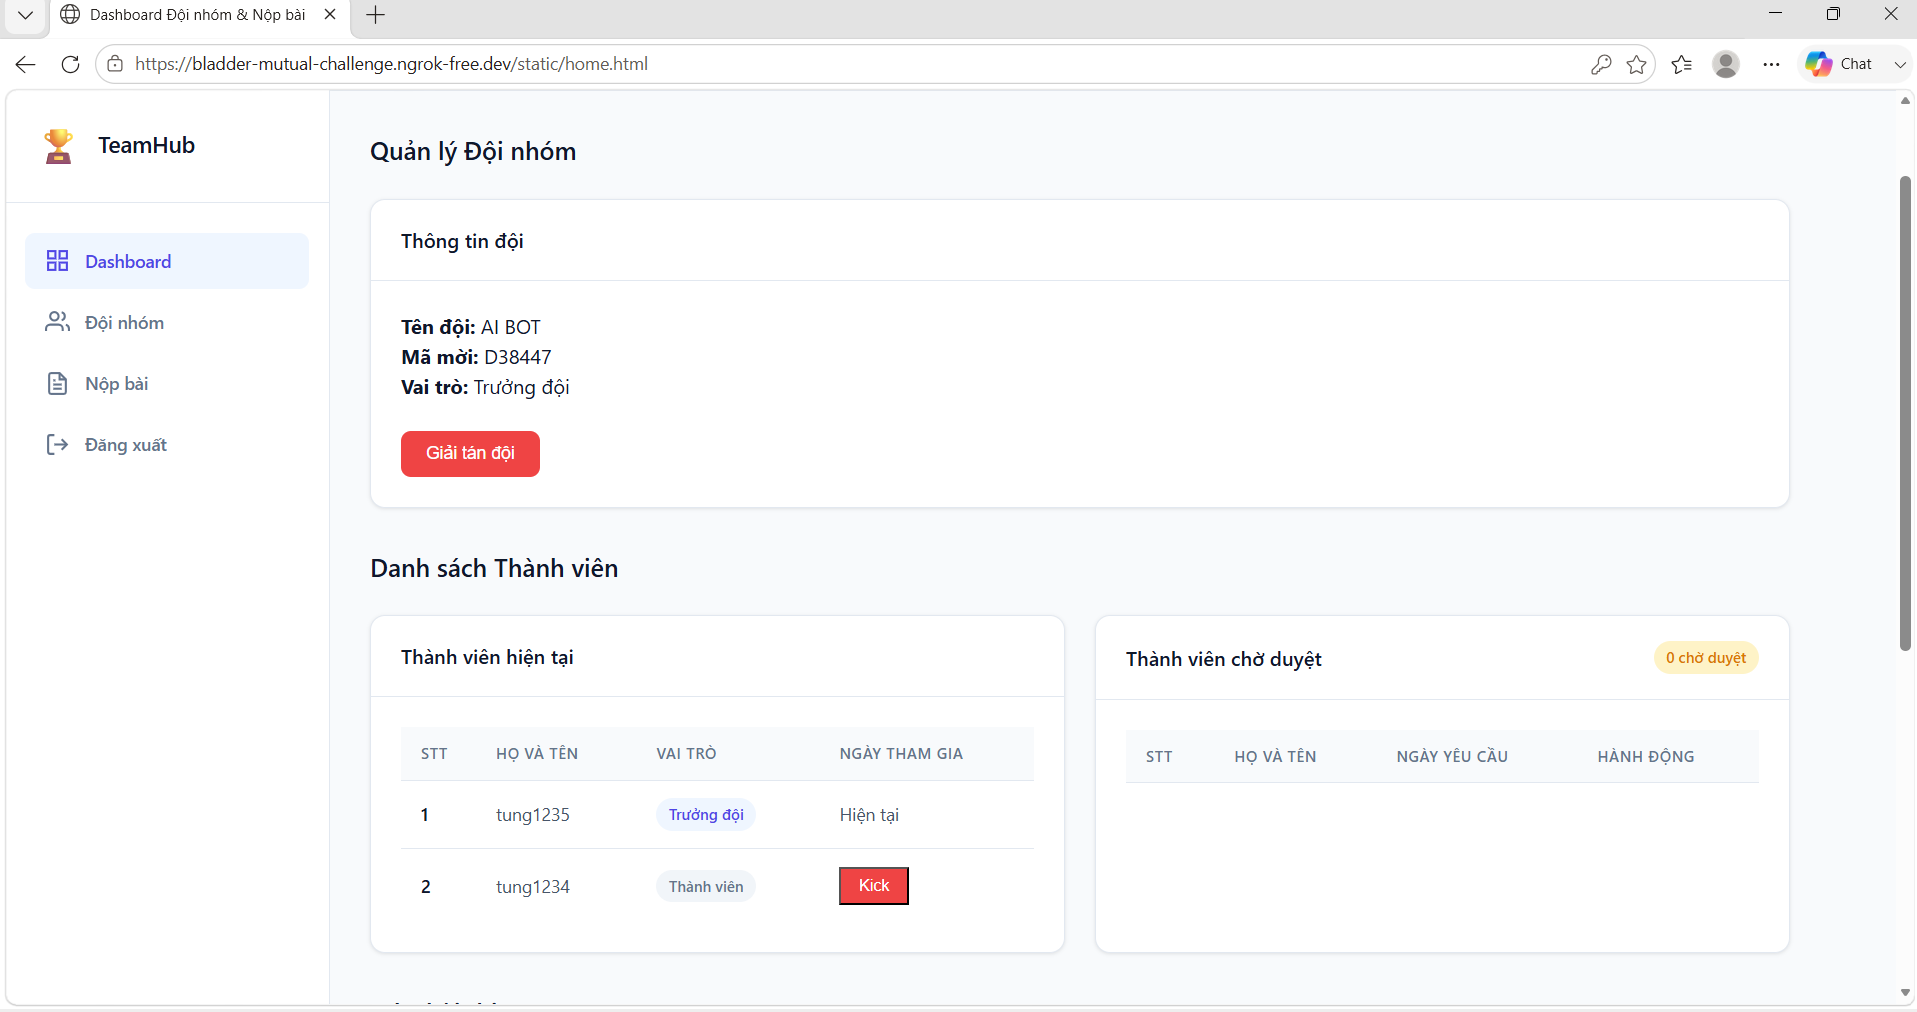
\includegraphics[width=0.82\textwidth]{images/approve_member.png}
	\caption{Kiểm thử TC-MEMBER-03}
	\label{fig:approve-member}
\end{figure}

%%%%%%%%%%%%%%%%%%%%%%%%%%%%%%%%%%%%%%%%%%%%%%%%%%%%%%%%%%%%%%%%%%%%%%%%%%%%%%
\subsection{TC-MEMBER-04: Loại thành viên khỏi đội}

\begin{table}[H]
	\centering
	\caption{Test Case TC-MEMBER-04}
	\label{tab:tc-member04}
	\renewcommand{\arraystretch}{1.3}
	
	\begin{tabular}{|p{4cm}|p{10cm}|}
		\hline
		\textbf{Thuộc tính} & \textbf{Nội dung} \\ \hline
		
		Test ID &
		TC-MEMBER-04
		\\ \hline
		
		Chức năng &
		Kick thành viên
		\\ \hline
		
		Mục tiêu &
		Kiểm tra Leader có quyền loại thành viên khỏi đội.
		\\ \hline
		
		Điều kiện tiên quyết &
		Đội có từ hai thành viên trở lên.
		\\ \hline
		
		Các bước thực hiện &
		Nhấn nút "Kick".
		\\ \hline
		
		Kết quả mong đợi &
		Thành viên bị xóa khỏi đội.
		\\ \hline
		
		Kết quả thực tế &
		Danh sách thành viên được cập nhật chính xác.
		\\ \hline
		
		Trạng thái &
		\textbf{PASS}
		\\ \hline
		
	\end{tabular}
\end{table}

\begin{figure}[H]
	\centering
	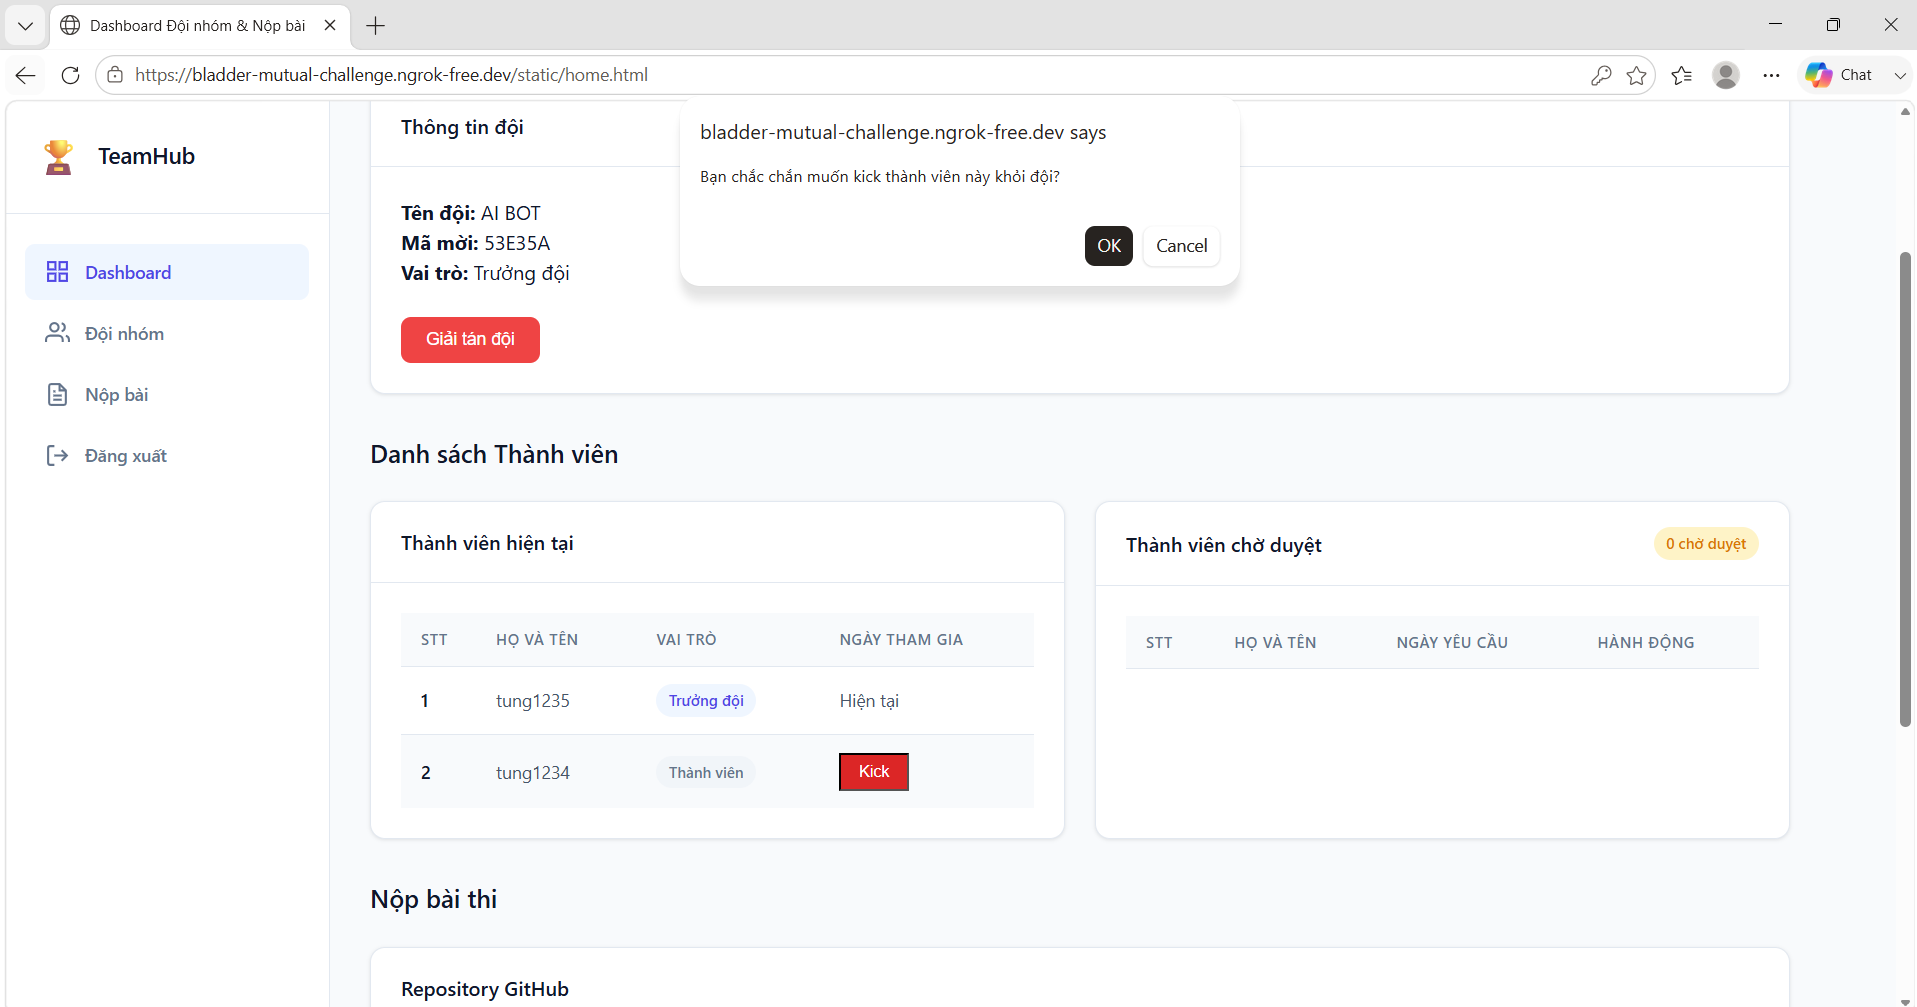
\includegraphics[width=0.82\textwidth]{images/kick_member.png}
	\caption{Kiểm thử TC-MEMBER-04}
	\label{fig:kick-member}
\end{figure}
%%%%%%%%%%%%%%%%%%%%%%%%%%%%%%%%%%%%%%%%%%%%%%%%%%%%%%%%%%%%%%%%%%%%%%%%%%%%%%
\section{Kiểm thử chức năng rời đội và giải tán đội}
%%%%%%%%%%%%%%%%%%%%%%%%%%%%%%%%%%%%%%%%%%%%%%%%%%%%%%%%%%%%%%%%%%%%%%%%%%%%%%

Sau khi đội được thành lập và các thành viên đã tham gia, hệ thống cho phép thành viên chủ động rời khỏi đội hoặc Trưởng đội giải tán toàn bộ đội khi không còn nhu cầu hoạt động. Hai chức năng này giúp bảo đảm dữ liệu của hệ thống luôn phản ánh đúng trạng thái thực tế của các đội thi.

Nhóm tiến hành kiểm thử hai chức năng trên nhằm đánh giá tính chính xác của cơ chế phân quyền, khả năng cập nhật dữ liệu và giao diện người dùng sau khi thực hiện thao tác.

%%%%%%%%%%%%%%%%%%%%%%%%%%%%%%%%%%%%%%%%%%%%%%%%%%%%%%%%%%%%%%%%%%%%%%%%%%%%%%
\subsection{TC-TEAM-04: Thành viên rời đội}

\begin{table}[H]
	\centering
	\caption{Test Case TC-TEAM-04}
	\label{tab:tc-team04}
	\renewcommand{\arraystretch}{1.3}
	
	\begin{tabular}{|p{4cm}|p{10cm}|}
		
		\hline
		\textbf{Thuộc tính} &
		\textbf{Nội dung}
		\\ \hline
		
		Test ID &
		TC-TEAM-04
		\\ \hline
		
		Chức năng &
		Rời đội
		\\ \hline
		
		Mục tiêu &
		Kiểm tra thành viên có thể chủ động rời khỏi đội.
		\\ \hline
		
		Điều kiện tiên quyết &
		Người dùng đang là thành viên của một đội.
		\\ \hline
		
		Các bước thực hiện &
		1. Đăng nhập.
		
		2. Chọn mục Cài đặt.
		
		3. Nhấn nút "Rời đội".
		
		4. Xác nhận thao tác.
		\\ \hline
		
		Kết quả mong đợi &
		Thành viên được xóa khỏi đội và quay về trạng thái chưa có đội.
		\\ \hline
		
		Kết quả thực tế &
		Hệ thống cập nhật dữ liệu thành công và Dashboard hiển thị giao diện chưa có đội.
		\\ \hline
		
		Trạng thái &
		\textbf{PASS}
		\\ \hline
		
	\end{tabular}
	
\end{table}

\begin{figure}[H]
	\centering
	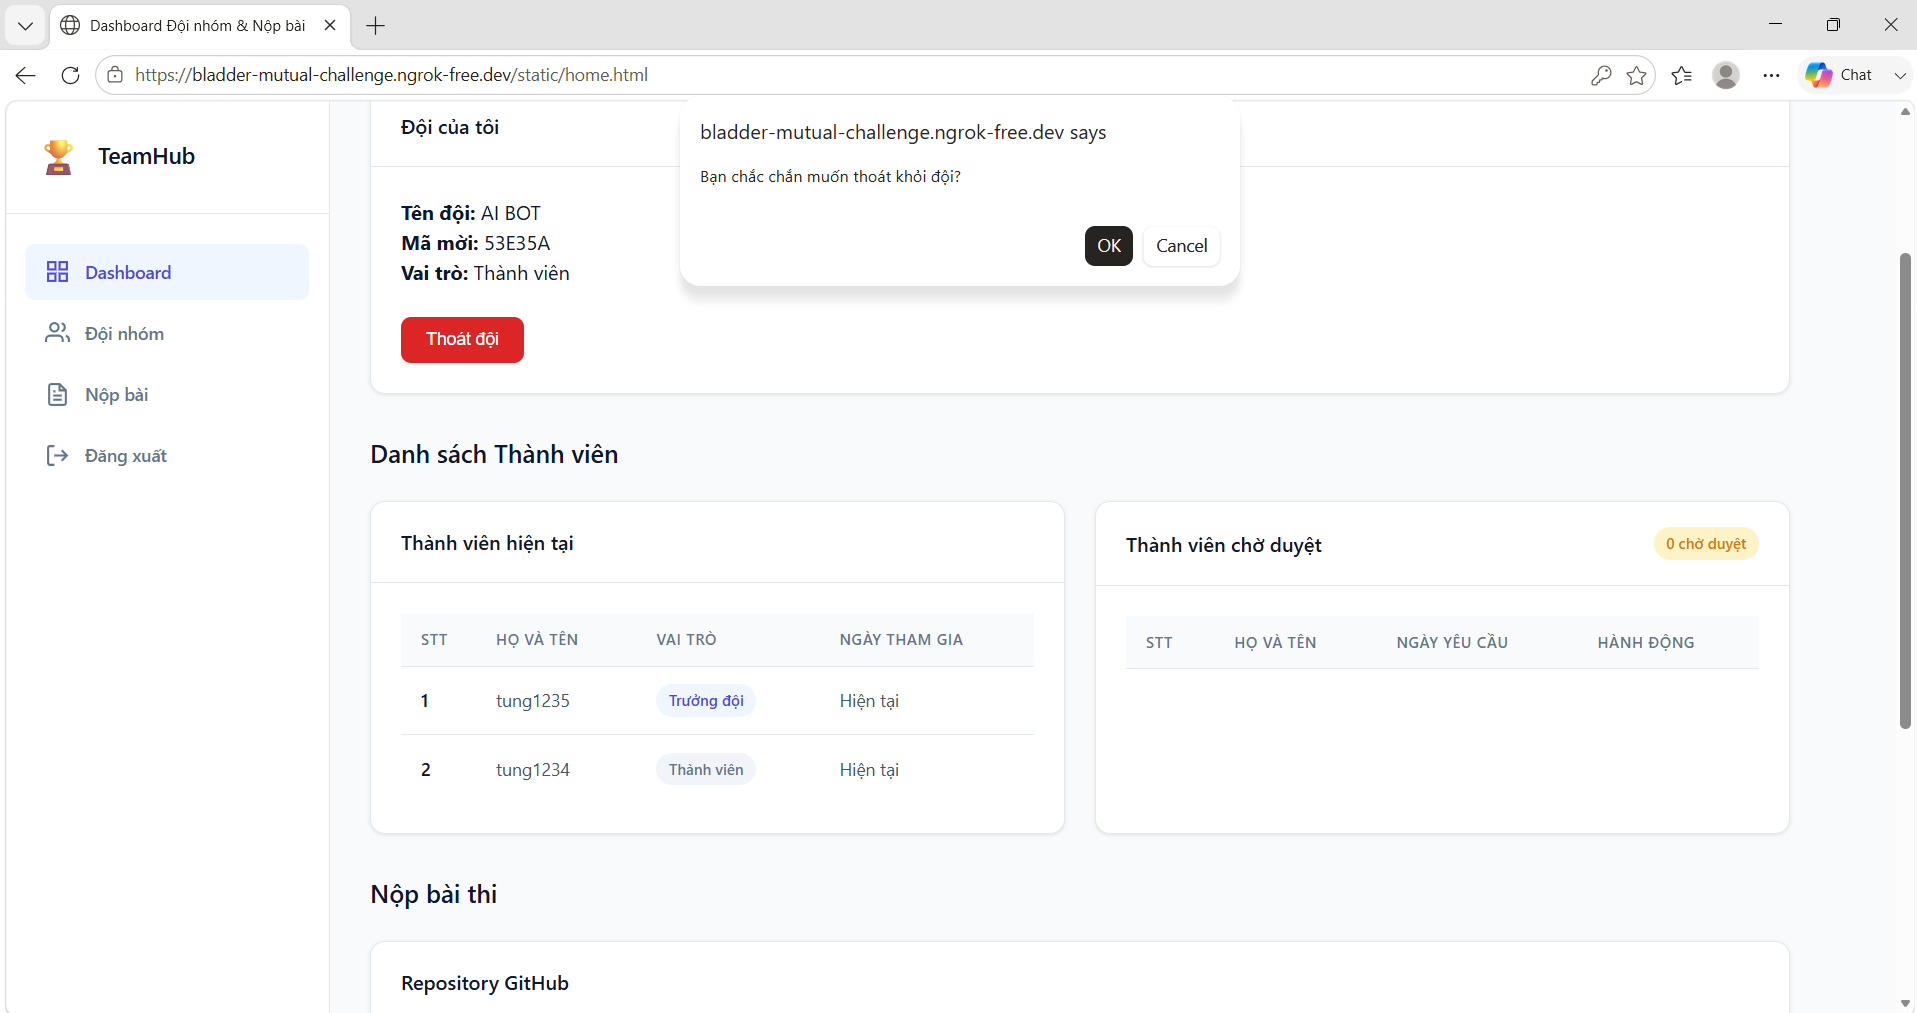
\includegraphics[width=0.75\textwidth]{images/leave_team_confirm.png}
	\caption{Xác nhận rời khỏi đội}
	\label{fig:leave-confirm}
\end{figure}

\begin{figure}[H]
	\centering
	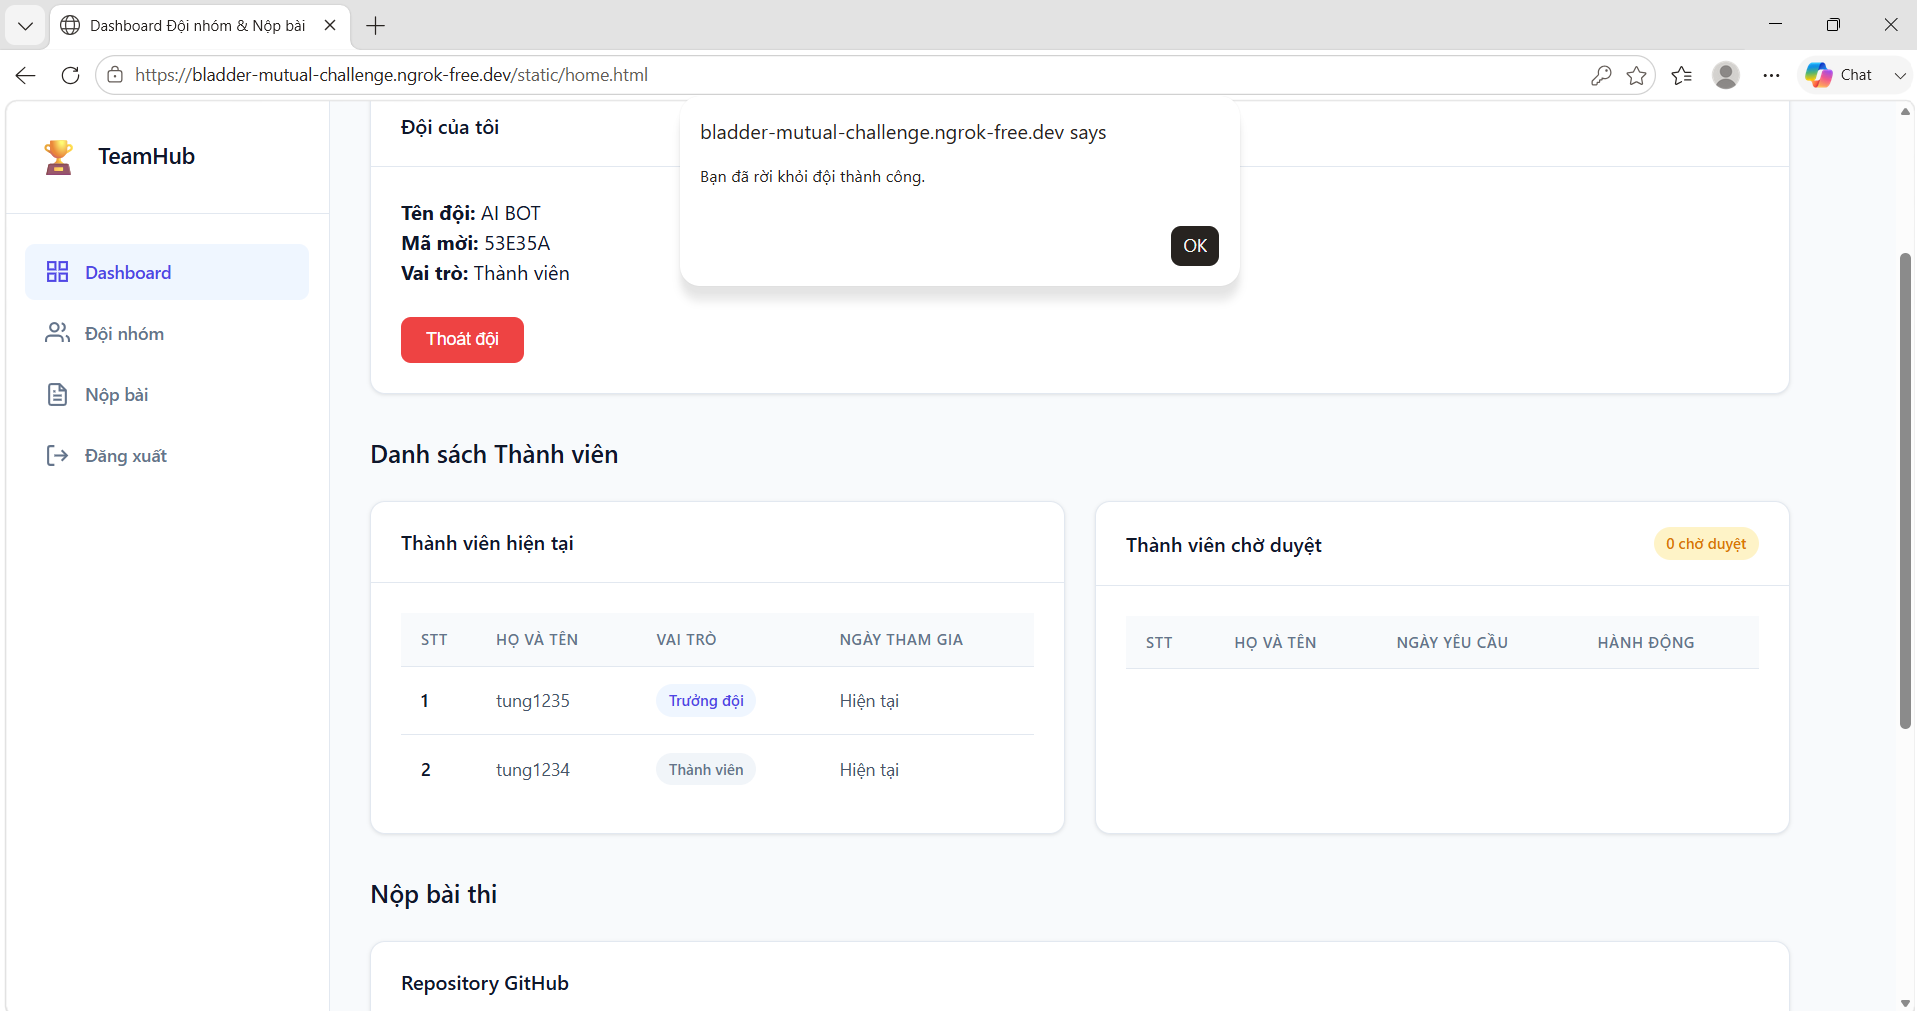
\includegraphics[width=0.80\textwidth]{images/leave_team_success.png}
	\caption{Kết quả sau khi rời khỏi đội}
	\label{fig:leave-success}
\end{figure}

Sau khi xác nhận, hệ thống cập nhật cơ sở dữ liệu, loại bỏ thành viên khỏi đội và giao diện Dashboard chuyển về trạng thái ban đầu.

%%%%%%%%%%%%%%%%%%%%%%%%%%%%%%%%%%%%%%%%%%%%%%%%%%%%%%%%%%%%%%%%%%%%%%%%%%%%%%
\subsection{TC-TEAM-05: Trưởng đội giải tán đội}

\begin{table}[H]
	\centering
	\caption{Test Case TC-TEAM-05}
	\label{tab:tc-team05}
	\renewcommand{\arraystretch}{1.3}
	
	\begin{tabular}{|p{4cm}|p{10cm}|}
		
		\hline
		\textbf{Thuộc tính} &
		\textbf{Nội dung}
		\\ \hline
		
		Test ID &
		TC-TEAM-05
		\\ \hline
		
		Chức năng &
		Giải tán đội
		\\ \hline
		
		Mục tiêu &
		Kiểm tra Leader có thể giải tán đội.
		\\ \hline
		
		Điều kiện tiên quyết &
		Người dùng là Trưởng đội.
		\\ \hline
		
		Các bước thực hiện &
		1. Đăng nhập.
		
		2. Chọn mục Cài đặt.
		
		3. Nhấn nút "Giải tán đội".
		
		4. Xác nhận thao tác.
		\\ \hline
		
		Kết quả mong đợi &
		Đội bị xóa khỏi cơ sở dữ liệu, tất cả thành viên không còn thuộc đội.
		\\ \hline
		
		Kết quả thực tế &
		Đội được xóa thành công và Dashboard trở về trạng thái chưa có đội.
		\\ \hline
		
		Trạng thái &
		\textbf{PASS}
		\\ \hline
		
	\end{tabular}
	
\end{table}

\begin{figure}[H]
	\centering
	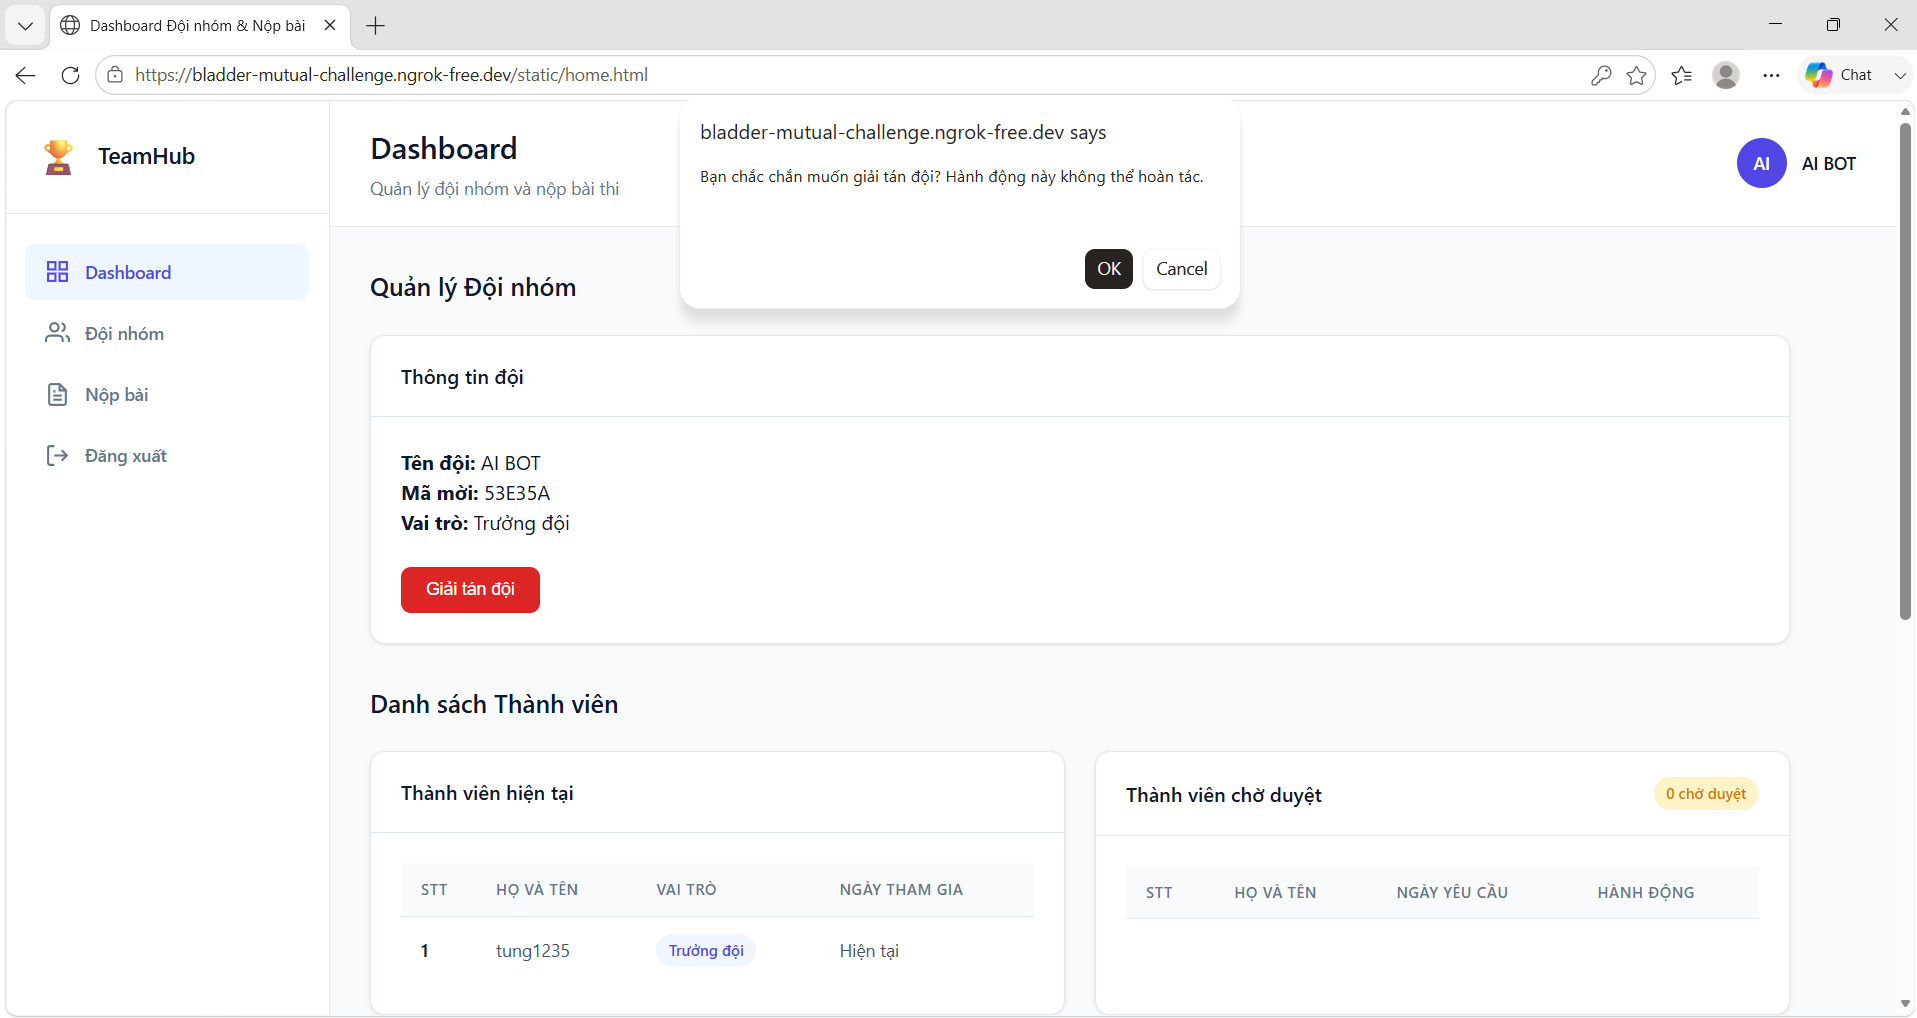
\includegraphics[width=0.75\textwidth]{images/disband_team_confirm.png}
	\caption{Xác nhận giải tán đội}
	\label{fig:disband-confirm}
\end{figure}

\begin{figure}[H]
	\centering
	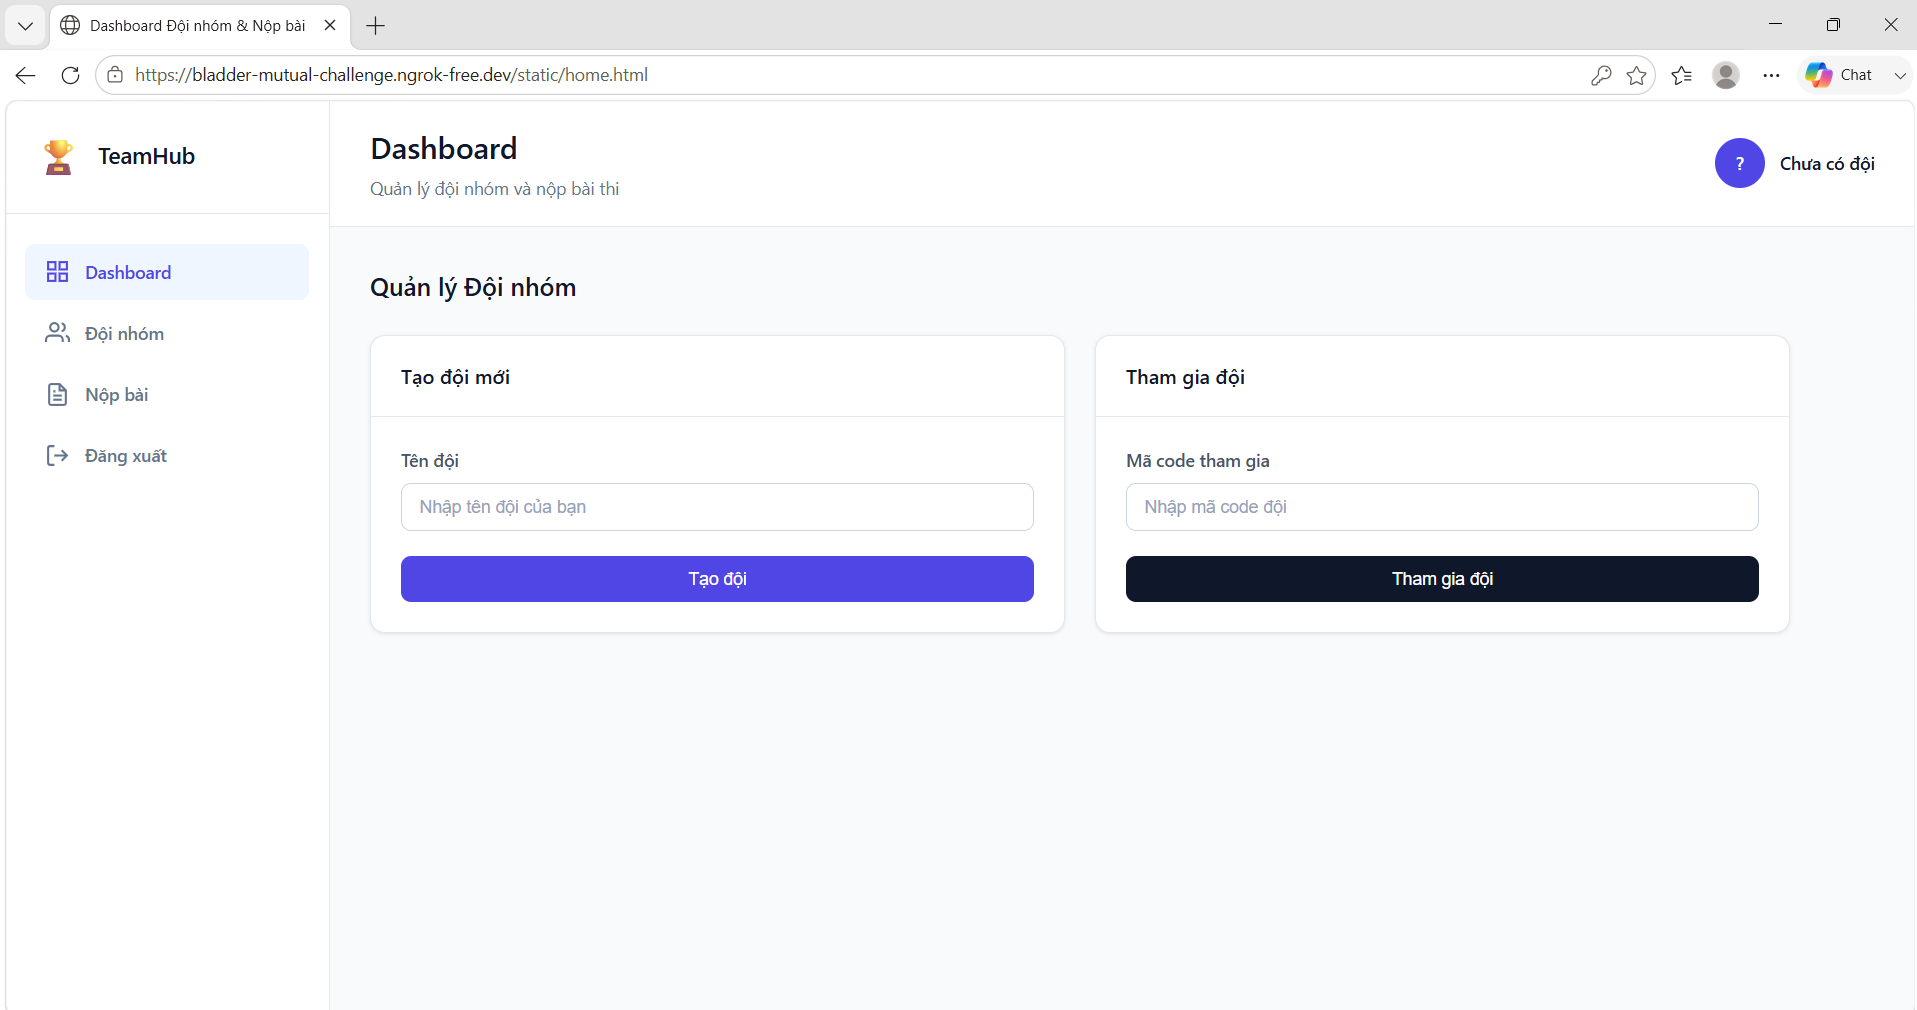
\includegraphics[width=0.80\textwidth]{images/disband_team_success.png}
	\caption{Kết quả sau khi giải tán đội}
	\label{fig:disband-success}
\end{figure}

Kết quả kiểm thử cho thấy hệ thống thực hiện đúng quy tắc phân quyền, chỉ Trưởng đội mới có quyền giải tán đội. Sau khi thao tác hoàn tất, dữ liệu đội được xóa khỏi cơ sở dữ liệu và giao diện người dùng được cập nhật chính xác.
%%%%%%%%%%%%%%%%%%%%%%%%%%%%%%%%%%%%%%%%%%%%%%%%%%%%%%%%%%%%%%%%%%%%%%%%%%%%%%
\section{Kiểm thử chức năng nộp bài dự thi}
%%%%%%%%%%%%%%%%%%%%%%%%%%%%%%%%%%%%%%%%%%%%%%%%%%%%%%%%%%%%%%%%%%%%%%%%%%%%%%

Sau khi hoàn thành việc thành lập đội và phát triển dự án, Trưởng đội thực hiện chức năng nộp bài thông qua đường dẫn GitHub của dự án. Chức năng này cho phép hệ thống lưu trữ liên kết GitHub của đội để phục vụ cho quá trình đánh giá và chấm điểm.

Trong quá trình kiểm thử, nhóm tiến hành đánh giá việc nộp bài với đường dẫn hợp lệ và trường hợp cập nhật lại đường dẫn sau khi đã nộp.

%%%%%%%%%%%%%%%%%%%%%%%%%%%%%%%%%%%%%%%%%%%%%%%%%%%%%%%%%%%%%%%%%%%%%%%%%%%%%%
\subsection{TC-SUBMIT-01: Nộp bài thành công}

\begin{table}[H]
	\centering
	\caption{Test Case TC-SUBMIT-01}
	\label{tab:tc-submit01}
	\renewcommand{\arraystretch}{1.3}
	
	\begin{tabular}{|p{4cm}|p{10cm}|}
		\hline
		\textbf{Thuộc tính} & \textbf{Nội dung} \\ \hline
		
		Test ID &
		TC-SUBMIT-01
		\\ \hline
		
		Chức năng &
		Nộp bài dự thi
		\\ \hline
		
		Mục tiêu &
		Kiểm tra khả năng nộp liên kết GitHub của đội.
		\\ \hline
		
		Điều kiện tiên quyết &
		Người dùng là Trưởng đội và đội đã được tạo thành công.
		\\ \hline
		
		Dữ liệu đầu vào &
		https://github.com/Quang-Tri/SEAL-Hackathon-Management
		\\ \hline
		
		Các bước thực hiện &
		1. Mở mục Nộp bài.
		
		2. Nhập đường dẫn GitHub.
		
		3. Nhấn nút Nộp bài.
		\\ \hline
		
		Kết quả mong đợi &
		Hệ thống lưu đường dẫn GitHub vào cơ sở dữ liệu và hiển thị thông báo thành công.
		\\ \hline
		
		Kết quả thực tế &
		Liên kết GitHub được lưu thành công và hiển thị thông báo "Nộp bài thành công".
		\\ \hline
		
		Trạng thái &
		\textbf{PASS}
		\\ \hline
		
	\end{tabular}
\end{table}

\begin{figure}[H]
	\centering
	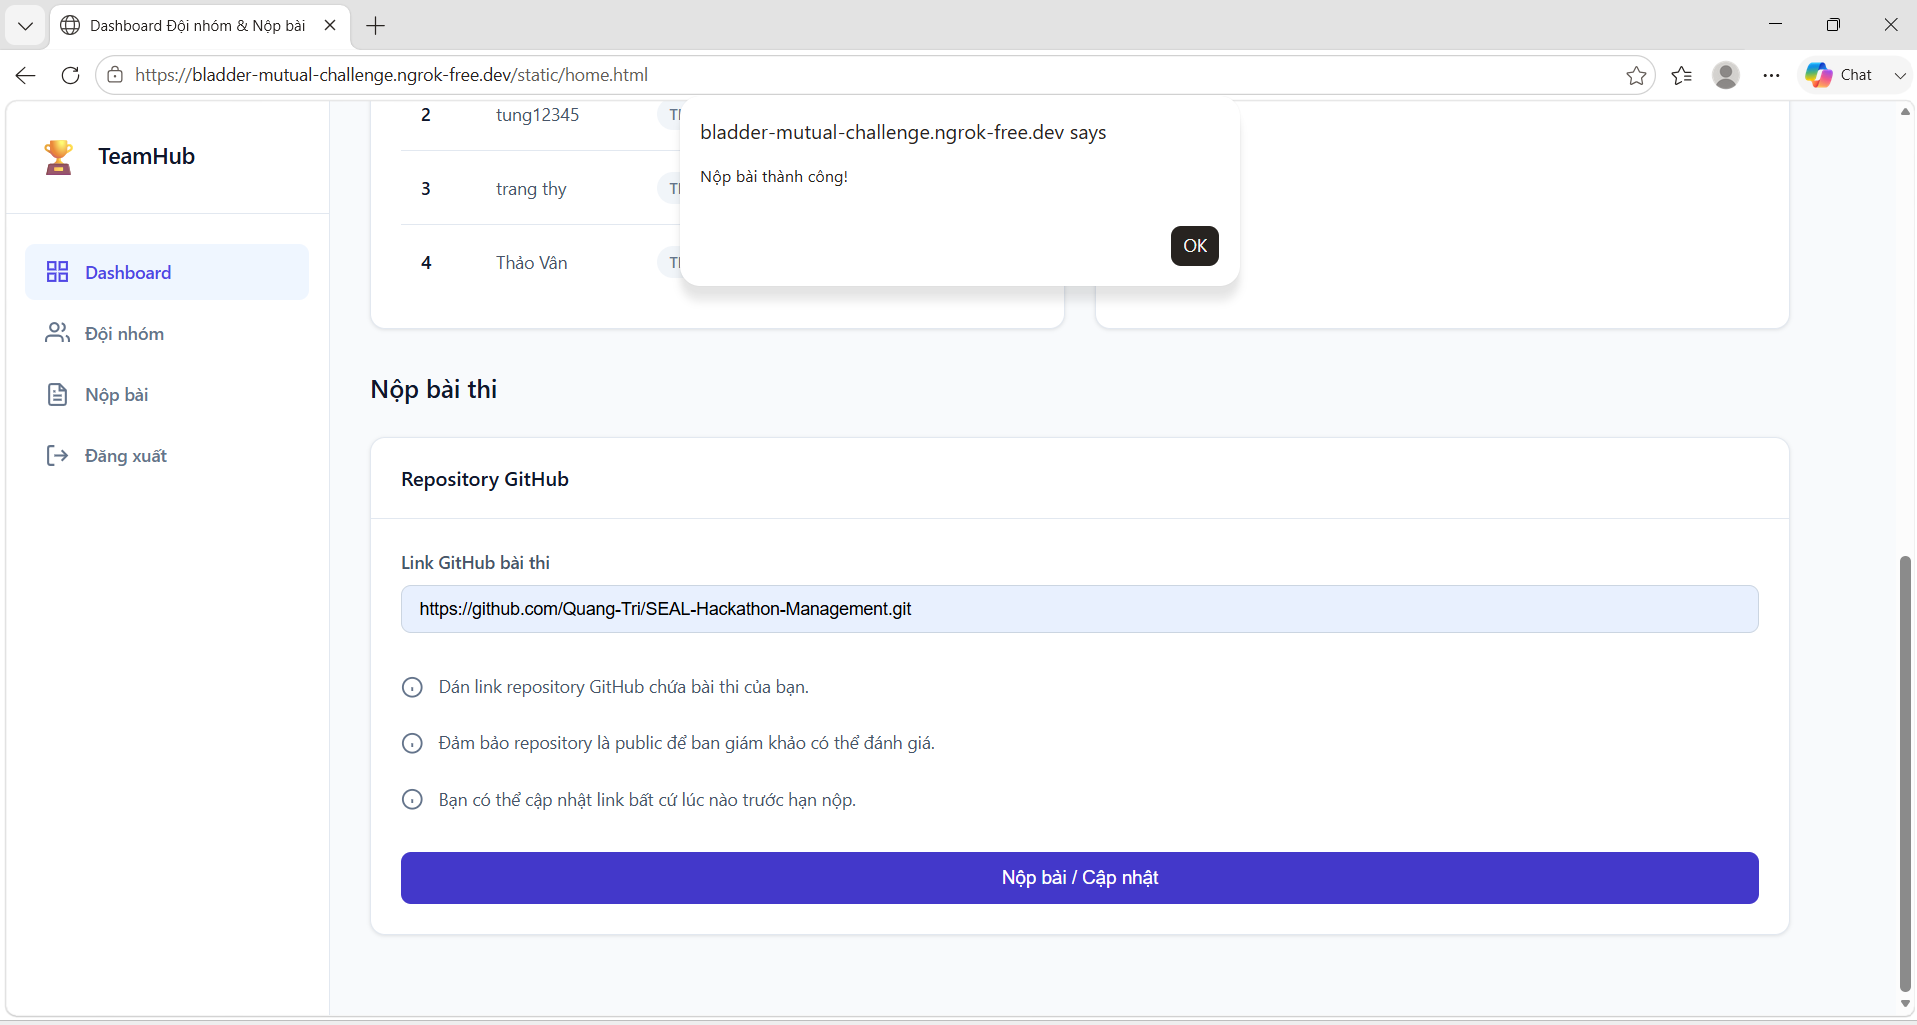
\includegraphics[width=0.82\textwidth]{images/submit_github_success.png}
	\caption{Kết quả kiểm thử TC-SUBMIT-01}
	\label{fig:submit-success}
\end{figure}

Kết quả kiểm thử cho thấy hệ thống đã tiếp nhận và lưu chính xác đường dẫn GitHub của đội vào cơ sở dữ liệu.

%%%%%%%%%%%%%%%%%%%%%%%%%%%%%%%%%%%%%%%%%%%%%%%%%%%%%%%%%%%%%%%%%%%%%%%%%%%%%%
\subsection{TC-SUBMIT-02: Cập nhật lại đường dẫn GitHub}

\begin{table}[H]
	\centering
	\caption{Test Case TC-SUBMIT-02}
	\label{tab:tc-submit02}
	\renewcommand{\arraystretch}{1.3}
	
	\begin{tabular}{|p{4cm}|p{10cm}|}
		\hline
		\textbf{Thuộc tính} & \textbf{Nội dung} \\ \hline
		
		Test ID &
		TC-SUBMIT-02
		\\ \hline
		
		Chức năng &
		Cập nhật bài nộp
		\\ \hline
		
		Mục tiêu &
		Kiểm tra khả năng cập nhật lại liên kết GitHub khi đội đã nộp bài trước đó.
		\\ \hline
		
		Điều kiện tiên quyết &
		Đội đã tồn tại một bài nộp.
		\\ \hline
		
		Dữ liệu đầu vào &
		https://github.com/Quang-Tri/SEAL-Hackathon-Management
		\\ \hline
		
		Các bước thực hiện &
		1. Truy cập mục Nộp bài.
		
		2. Thay đổi đường dẫn GitHub.
		
		3. Nhấn nút Cập nhật.
		\\ \hline
		
		Kết quả mong đợi &
		Hệ thống cập nhật đường dẫn GitHub mới và ghi đè dữ liệu cũ.
		\\ \hline
		
		Kết quả thực tế &
		Đường dẫn GitHub được cập nhật thành công.
		\\ \hline
		
		Trạng thái &
		\textbf{PASS}
		\\ \hline
		
	\end{tabular}
\end{table}

\begin{figure}[H]
	\centering
	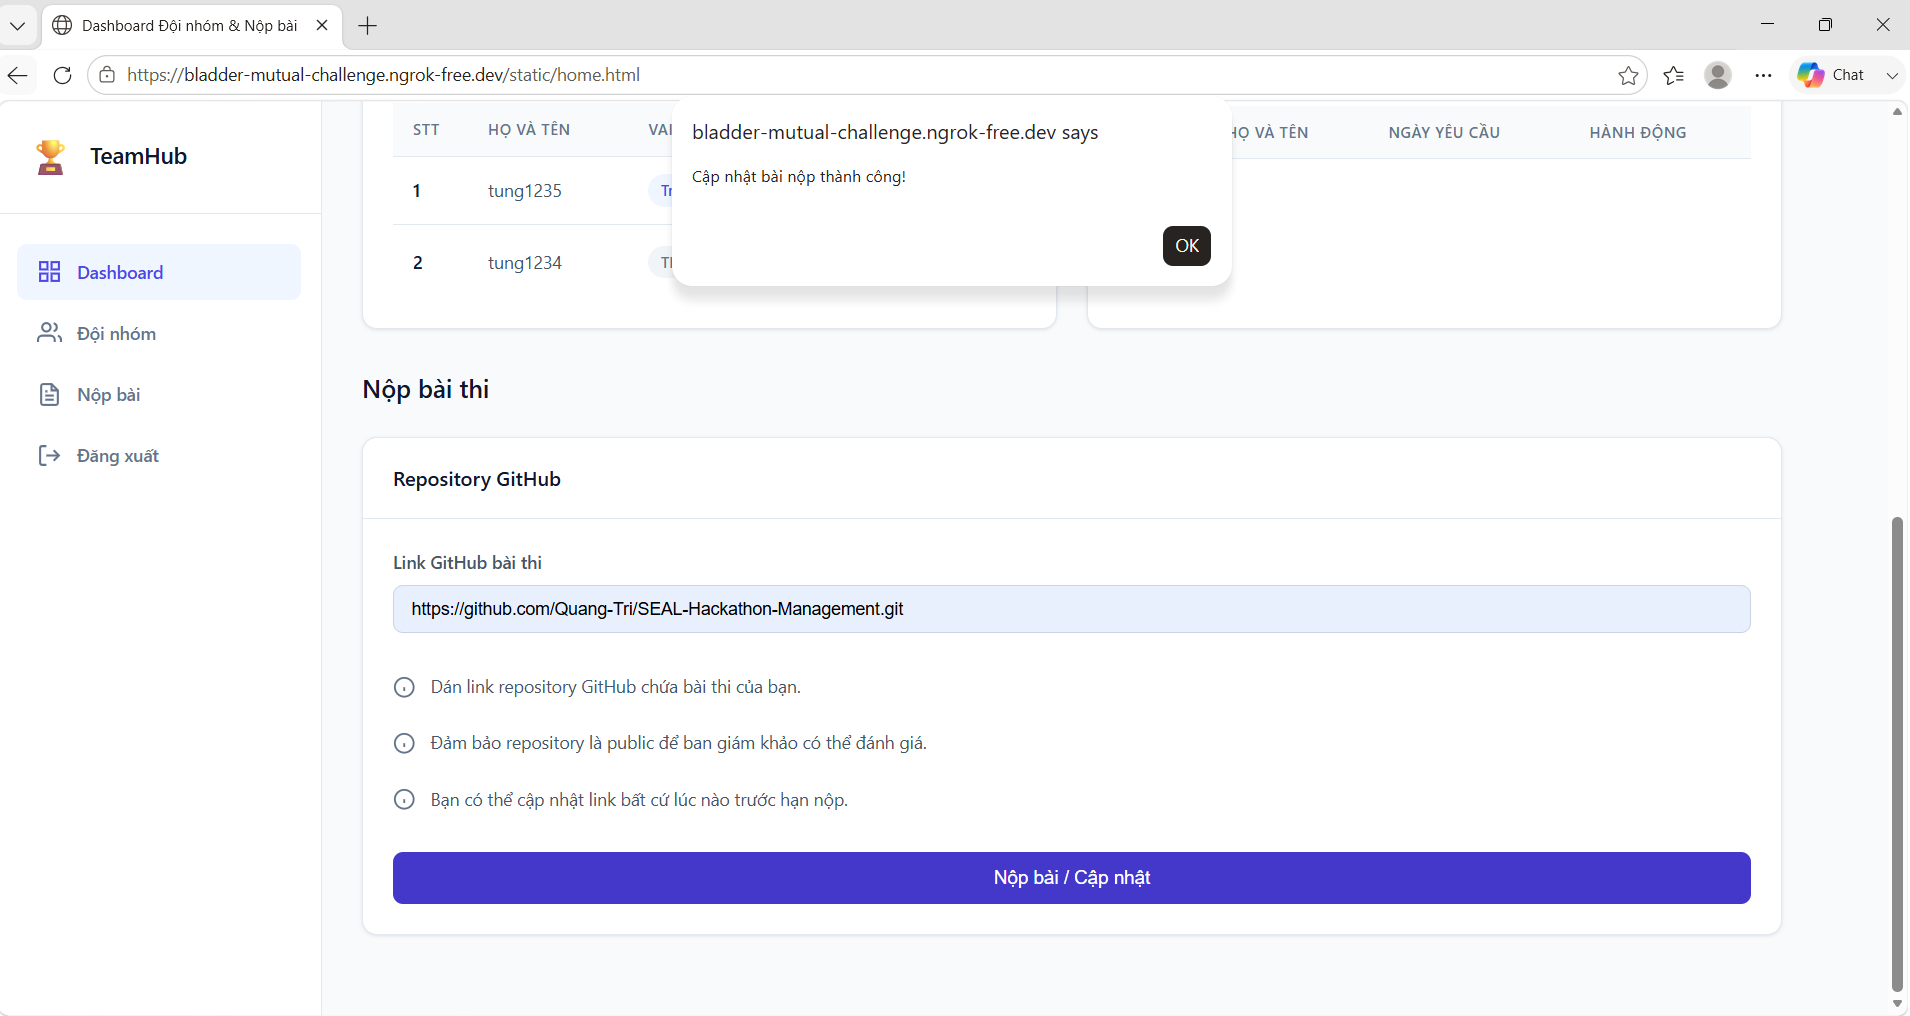
\includegraphics[width=0.82\textwidth]{images/update_github_success.png}
	\caption{Kết quả kiểm thử TC-SUBMIT-02}
	\label{fig:update-submit}
\end{figure}

Hệ thống cho phép cập nhật bài nộp nhiều lần mà không làm phát sinh bản ghi trùng lặp trong cơ sở dữ liệu.

%%%%%%%%%%%%%%%%%%%%%%%%%%%%%%%%%%%%%%%%%%%%%%%%%%%%%%%%%%%%%%%%%%%%%%%%%%%%%%
\subsection{Đánh giá chức năng}

Thông qua các trường hợp kiểm thử trên, chức năng nộp bài của hệ thống đã đáp ứng đúng yêu cầu nghiệp vụ. Hệ thống lưu trữ và cập nhật đường dẫn GitHub chính xác, đồng thời phản hồi đầy đủ trạng thái cho người sử dụng sau mỗi thao tác. Điều này giúp Ban tổ chức có thể dễ dàng truy cập và đánh giá mã nguồn của các đội tham gia cuộc thi.
%%%%%%%%%%%%%%%%%%%%%%%%%%%%%%%%%%%%%%%%%%%%%%%%%%%%%%%%%%%%%%%%%%%%%%%%%%%%%%
\section{Tổng hợp kết quả kiểm thử}
%%%%%%%%%%%%%%%%%%%%%%%%%%%%%%%%%%%%%%%%%%%%%%%%%%%%%%%%%%%%%%%%%%%%%%%%%%%%%%

Sau khi hoàn thành quá trình kiểm thử, nhóm tiến hành tổng hợp kết quả đối với các chức năng chính của hệ thống. Việc kiểm thử được thực hiện dựa trên các Test Case đã xây dựng, bao gồm cả trường hợp hợp lệ và không hợp lệ nhằm đánh giá đầy đủ khả năng xử lý của hệ thống.

Bảng \ref{tab:test-summary} trình bày kết quả tổng hợp các chức năng đã được kiểm thử.

\begin{table}[H]
	\centering
	\caption{Tổng hợp kết quả kiểm thử}
	\label{tab:test-summary}
	\renewcommand{\arraystretch}{1.3}
	
	\begin{tabular}{|c|p{7cm}|c|c|}
		\hline
		
		\textbf{STT} &
		\textbf{Chức năng} &
		\textbf{Số Test Case} &
		\textbf{Kết quả}
		
		\\
		\hline
		
		1 &
		Đăng ký tài khoản &
		3 &
		PASS
		
		\\
		\hline
		
		2 &
		Đăng nhập hệ thống &
		2 &
		PASS
		
		\\
		\hline
		
		3 &
		Quản lý đội nhóm &
		3 &
		PASS
		
		\\
		\hline
		
		4 &
		Quản lý thành viên &
		4 &
		PASS
		
		\\
		\hline
		
		5 &
		Rời đội và giải tán đội &
		2 &
		PASS
		
		\\
		\hline
		
		6 &
		Nộp bài dự thi &
		2 &
		PASS
		
		\\
		\hline
		
		\textbf{Tổng cộng} &
		&
		\textbf{16}
		&
		\textbf{PASS}
		
		\\
		\hline
		
	\end{tabular}
	
\end{table}

Kết quả kiểm thử cho thấy toàn bộ các chức năng chính của hệ thống đều hoạt động đúng theo yêu cầu đã đặt ra. Các chức năng được triển khai ổn định, dữ liệu được cập nhật chính xác giữa giao diện người dùng và cơ sở dữ liệu, đồng thời cơ chế phân quyền giữa Trưởng đội và Thành viên được thực hiện đúng theo thiết kế.

%%%%%%%%%%%%%%%%%%%%%%%%%%%%%%%%%%%%%%%%%%%%%%%%%%%%%%%%%%%%%%%%%%%%%%%%%%%%%%
\section{Các lỗi phát hiện trong quá trình phát triển}
%%%%%%%%%%%%%%%%%%%%%%%%%%%%%%%%%%%%%%%%%%%%%%%%%%%%%%%%%%%%%%%%%%%%%%%%%%%%%%

Trong quá trình xây dựng và kiểm thử hệ thống, nhóm đã phát hiện và khắc phục nhiều lỗi ảnh hưởng đến quá trình vận hành. Việc ghi nhận và xử lý các lỗi này góp phần nâng cao chất lượng của hệ thống trước khi hoàn thiện.

\begin{table}[H]
	\centering
	\caption{Các lỗi đã phát hiện và khắc phục}
	\label{tab:bug-summary}
	\renewcommand{\arraystretch}{1.3}
	
	\begin{tabular}{|c|p{5cm}|p{4cm}|p{3cm}|}
		
		\hline
		
		\textbf{STT} &
		\textbf{Lỗi phát hiện} &
		\textbf{Nguyên nhân} &
		\textbf{Trạng thái}
		
		\\
		\hline
		
		1 &
		Không thể đăng ký tài khoản mới &
		Kiểm tra Username và Email chưa đầy đủ &
		Đã sửa
		
		\\
		\hline
		
		2 &
		Dashboard hiển thị dữ liệu mẫu &
		Chưa lấy dữ liệu từ API &
		Đã sửa
		
		\\
		\hline
		
		3 &
		Người dùng chưa có đội vẫn hiển thị danh sách thành viên &
		Điều kiện hiển thị giao diện chưa chính xác &
		Đã sửa
		
		\\
		\hline
		
		4 &
		Leader không thể Kick thành viên &
		API và Frontend chưa đồng bộ &
		Đã sửa
		
		\\
		\hline
		
		5 &
		Đăng xuất không hoạt động &
		Chưa xóa JWT Token trong Local Storage &
		Đã sửa
		
		\\
		\hline
		
		6 &
		Giao diện Dashboard chưa cập nhật sau khi tạo đội &
		Chưa reload dữ liệu từ API &
		Đã sửa
		
		\\
		\hline
		
	\end{tabular}
	
\end{table}

Qua quá trình kiểm thử và hiệu chỉnh, các lỗi phát hiện đều đã được nhóm xử lý và kiểm thử lại. Sau khi khắc phục, hệ thống hoạt động ổn định và đáp ứng đúng các yêu cầu chức năng đã đề ra.

%%%%%%%%%%%%%%%%%%%%%%%%%%%%%%%%%%%%%%%%%%%%%%%%%%%%%%%%%%%%%%%%%%%%%%%%%%%%%%
\section{Đánh giá chương}
%%%%%%%%%%%%%%%%%%%%%%%%%%%%%%%%%%%%%%%%%%%%%%%%%%%%%%%%%%%%%%%%%%%%%%%%%%%%%%

Thông qua quá trình kiểm thử, nhóm đã đánh giá toàn diện các chức năng quan trọng của hệ thống SEAL Hackathon Management System. Kết quả cho thấy các chức năng chính như đăng ký, đăng nhập, quản lý đội, quản lý thành viên và nộp bài đều hoạt động đúng theo yêu cầu nghiệp vụ.

Bên cạnh việc kiểm thử các trường hợp hợp lệ, nhóm cũng thực hiện nhiều trường hợp kiểm thử không hợp lệ nhằm đánh giá khả năng xử lý lỗi của hệ thống. Các thông báo lỗi được hiển thị đầy đủ, dữ liệu được kiểm tra trước khi lưu vào cơ sở dữ liệu và cơ chế phân quyền được thực hiện chính xác giữa Trưởng đội và Thành viên.

Quá trình kiểm thử cũng giúp nhóm phát hiện một số lỗi trong giai đoạn phát triển như lỗi đồng bộ dữ liệu Dashboard, lỗi đăng xuất, lỗi Kick thành viên và lỗi hiển thị giao diện. Sau khi được khắc phục và kiểm thử lại, các chức năng đều hoạt động ổn định.

Nhìn chung, hệ thống đã đáp ứng các yêu cầu của đề tài, đảm bảo tính đúng đắn của các chức năng cốt lõi và có thể tiếp tục được mở rộng trong các phiên bản tiếp theo như bổ sung chức năng chấm điểm tự động, gửi thông báo thời gian thực và triển khai trên môi trường Cloud.